\documentclass[pdf]{beamer}

%\usepackage{lmodern}
\usepackage[font=scriptsize,skip=0pt,justification=justified,singlelinecheck=false]{caption}
%\usepackage{enumitem}
\usepackage{natbib}
\usepackage{bm}
\usepackage{mathtools}
\usepackage[makeroom]{cancel}

\usepackage{xcolor}
\usepackage{hyperref}

% Using underline
\usepackage{soul}

\usepackage{algorithm}
\usepackage{algpseudocode}
%\usepackage[ruled,vlined]{algorithm2e}
%\usepackage{clrscode3e}


%\usepackage{adjustbox}

%remove the icon
\setbeamertemplate{bibliography item}{}

%remove line breaks
\setbeamertemplate{bibliography entry title}{}
\setbeamertemplate{bibliography entry location}{}
\setbeamertemplate{bibliography entry note}{}
% Use number for caption
\setbeamertemplate{caption}[numbered]{}

\newtheorem{mydef}[theorem]{\Large \underline{\textbf{Definisi}}}

\makeatletter
\def\th@mystyle{%
    \normalfont % body font
    \setbeamercolor{block title example}{bg=blue,fg=white}
    \setbeamercolor{block body example}{bg=blue!20,fg=black}
    \def\inserttheoremblockenv{exampleblock}
  }
\makeatother
\theoremstyle{mystyle}
\newtheorem*{remark}{\textbf{Definition}}


% This file is a solution template for:

% - Talk at a conference/colloquium.
% - Talk length is about 20min.
% - Style is ornate.

% Copyright 2004 by Till Tantau <tantau@users.sourceforge.net>.
%
% In principle, this file can be redistributed and/or modified under
% the terms of the GNU Public License, version 2.
%
% However, this file is supposed to be a template to be modified
% for your own needs. For this reason, if you use this file as a
% template and not specifically distribute it as part of a another
% package/program, I grant the extra permission to freely copy and
% modify this file as you see fit and even to delete this copyright
% notice.  


\mode<presentation>
{
%  \usetheme{AnnArbor} % 
%	\usetheme{Frankfurt}
   \usetheme{Madrid}
  % or ...

%  \setbeamercovered{transparent}
  % or whatever (possibly just delete it)
}


\usepackage[english]{babel}
% or whatever

\usepackage[latin1]{inputenc}
% or whatever

\usepackage{times}
\usepackage[T1]{fontenc}
\usepackage{wasysym}

\usepackage{graphicx} % Necessary to use \scalebox

% Define absolute and norm
\DeclarePairedDelimiter\abs{\lvert}{\rvert}%
\DeclarePairedDelimiter\norm{\lVert}{\rVert}%

% ==============================
%       Redefine emphasize
% ==============================
\let\emph\relax % there's no \RedeclareTextFontCommand
\DeclareTextFontCommand{\emph}{\bfseries\em}


% Swap the definition of \abs* and \norm*, so that \abs
% and \norm resizes the size of the brackets, and the 
% starred version does not.
\makeatletter
\let\oldabs\abs
\def\abs{\@ifstar{\oldabs}{\oldabs*}}
%
\let\oldnorm\norm
\def\norm{\@ifstar{\oldnorm}{\oldnorm*}}
\makeatother

\usepackage{color}
\definecolor{myblue}{rgb}{.8,.8,1}
\usepackage{empheq}
% Or whatever. Note that the encoding and the font should match. If T1
% does not look nice, try deleting the line with the fontenc.

\newlength\mytemplen
\newsavebox\mytempbox

\makeatletter
\newcommand\mybluebox{%
    \@ifnextchar[%]
       {\@mybluebox}%
       {\@mybluebox[0pt]}}

\def\@mybluebox[#1]{%
    \@ifnextchar[%]
       {\@@mybluebox[#1]}%
       {\@@mybluebox[#1][0pt]}}

\def\@@mybluebox[#1][#2]#3{
    \sbox\mytempbox{#3}%
    \mytemplen\ht\mytempbox
    \advance\mytemplen #1\relax
    \ht\mytempbox\mytemplen
    \mytemplen\dp\mytempbox
    \advance\mytemplen #2\relax
    \dp\mytempbox\mytemplen
    \colorbox{myblue}{\hspace{1em}\usebox{\mytempbox}\hspace{1em}}}

\makeatother

\title[AI untuk Semua] % (optional, use only with long paper titles)
{\textbf{Pengenalan \textit{Artificial Intelligence}}}

\subtitle
{Jalur Peminatan \textit{AI Specialist}}

\author[Hendra Bunyamin] % (optional, use only with lots of authors)
{Hendra Bunyamin}
%{F.~Author\inst{1} \and S.~Another\inst{2}} --> original
% - Give the names in the same order as the appear in the paper.
% - Use the \inst{?} command only if the authors have different
%   affiliation.

\institute[ ] % (optional, but mostly needed)
{
%  \inst{1}%
  Program Studi Teknik Informatika\\
  Fakultas Teknologi Informasi\\
  Universitas Kristen Maranatha
%  \and
%  \inst{2}%
%  Department of Theoretical Philosophy\\
%  University of Elsewhere
}
% - Use the \inst command only if there are several affiliations.
% - Keep it simple, no one is interested in your street address.

%\date[CFP 2003] % (optional, should be abbreviation of conference name)
%{Conference on Fabulous Presentations, 2003}
% - Either use conference name or its abbreviation.
% - Not really informative to the audience, more for people (including
%   yourself) who are reading the slides online

\subject{Pengantar Teknologi Informasi}
% This is only inserted into the PDF information catalog. Can be left
% out. 

% If you have a file called "university-logo-filename.xxx", where xxx
% is a graphic format that can be processed by latex or pdflatex,
% resp., then you can add a logo as follows:

\pgfdeclareimage[height=1.5cm]{university-logo}{logo-mcu}
\logo{\pgfuseimage{university-logo}}


% Delete this, if you do not want the table of contents to pop up at
% the beginning of each subsection:
\AtBeginSection[]
{
  \begin{frame}<beamer>{Outline}
    \tableofcontents[currentsection,currentsection]
  \end{frame}
}


% If you wish to uncover everything in a step-wise fashion, uncomment
% the following command: 

%\beamerdefaultoverlayspecification{<+->}

\begin{document}

\begin{frame}
  \titlepage
\end{frame}

\begin{frame}{Outline}
  \tableofcontents
  % You might wish to add the option [pausesections]
\end{frame}


% Structuring a talk is a difficult task and the following structure
% may not be suitable. Here are some rules that apply for this
% solution: 

% - Exactly two or three sections (other than the summary).
% - At *most* three subsections per section.
% - Talk about 30s to 2min per frame. So there should be between about
%   15 and 30 frames, all told.

% - A conference audience is likely to know very little of what you
%   are going to talk about. So *simplify*!
% - In a 20min talk, getting the main ideas across is hard
%   enough. Leave out details, even if it means being less precise than
%   you think necessary.
% - If you omit details that are vital to the proof/implementation,
%   just say so once. Everybody will be happy with that.

%\begin{frame}{Make Titles Informative. Use Uppercase Letters.}{Subtitles are optional.}

\section{Introduction}
\begin{frame}{Introduction}
	\begin{figure}[!ht]
		\centering
		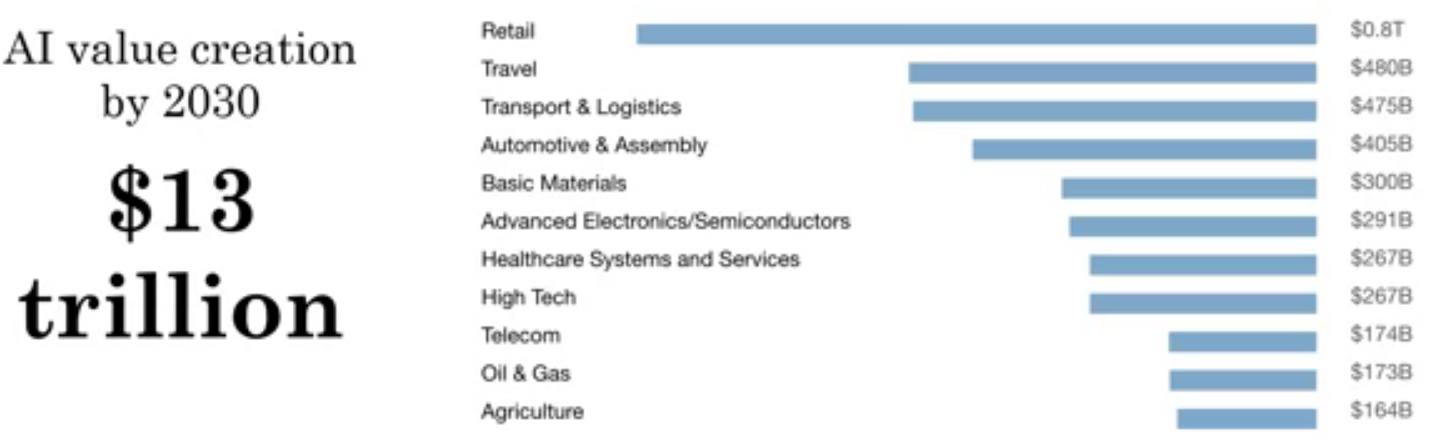
\includegraphics[scale=.225]{AI-value-creation}
		\caption{Source: McKinsey Global Institute~\citep{ng2019AIForEveryone}}
		\label{fig:ai-value-creation}
	\end{figure}
	\begin{align*}
	\$13 \text{ trillion } &= \$13 \times 10^{12} \\
	                       &= \text{Rp}183.000.000.000.000.000,- \\
                           &= 183 \text{ billiard}.	                       	
	\end{align*}	  
\end{frame}

\begin{frame}{Demystifying AI}
	Artificial Intelligence or \textbf{AI} can be divided into 2 as follows:
	\begin{itemize}
		\item<2-> \textbf{ANI} $\Rightarrow$ \textit{Artificial Narrow Intelligence}. \\
		\textbf{Examples}: smart speaker, self-driving car, web search, AI in farming and factories.
		\bigskip
		\item<3-> \textbf{AGI} $\Rightarrow$ \textit{Artificial General Intelligence}. \\
		\textbf{Examples}: Do anything or \textbf{even more} than a human can do.
	\end{itemize}
	\begin{center}
		\includegraphics<3->[scale=.125]{ex-machina} \qquad \includegraphics<3->[scale=.125]{upgrade}
	\end{center}
\end{frame}

\section{Machine Learning}
\begin{frame}{Machine Learning (1/2)}
	\begin{itemize}
		\item<2-> One of the tools that drive the significant progress of AI is \textbf{Machine Learning} (ML).
		\item<3-> \textbf{Machine Learning} is a set of methods that allow computers to \textit{learn from data} to \textit{make and improve predictions}, e.g., cancer, weekly sales, credit default~\citep{molnar2019}.  
		\begin{figure}[!ht]
			\centering
			\includegraphics<4->[scale=0.18]{images/programming-with-without-ml}
			\caption{\onslide<4-> A paradigm shift from "normal programming" to "indirect programming"}
		\end{figure}
	\end{itemize}		
\end{frame}

\begin{frame}{Machine Learning (2/2)}	
	The way a machine or computer learns can be categorized into several types~\citep{geron2019handson}:
	\begin{itemize}
		\item<2-> \textcolor <6-> {orange} {\textbf<6->{Supervised Learning}},
		\item<3-> Unsupervised Learning,
		\item<4-> Semi-supervised Learning, and
		\item<5-> Reinforcement learning
	\end{itemize}	
	
\end{frame}

\begin{frame}{Supervised Learning (1/2)}
	\begin{itemize}		
		\item A common type of of Machine Learning is a type of AI that learns from $A$ to $B$	or is often called \emph{Supervised Learning}.
		
		\bigskip
		
		\begin{center}
			
			\scalebox{2}{
				$A \longrightarrow B$
			} \\	
			\scalebox{1}{
				\qquad input \qquad \; \; output
			}							
		\end{center}
	\end{itemize}	
\end{frame}

\begin{frame}{Supervised Learning (2/2)}
	Consider the following examples \\
	(\textit{input} $A$ in \textbf{bold} and \textit{output} $B$ in italic)~\citep{trask2019grokking}:
	\begin{itemize}
		\item<2-> Using \textbf{pixels} of an image to detect the \textit{presence or absence of a cat}
		\item<3-> Using the \textbf{movies you've liked} to predict more \textit{movies you may like}
		\item<4-> Using someone's \textbf{words} to predict whether they're \textit{happy} or \textit{sad} 
		\item<5-> Using \textbf{weather sensor data} to predict the \textit{probability of rain}
		\item<6-> Using \textbf{car engine sensors} to predict the optimal tuning \textit{settings}
		\item<7-> Using \textbf{news data} to predict tomorrow's stock \textit{price}
		\item<8-> Using a raw \textbf{audio file} to predict a \textit{transcript} of the audio.
	\end{itemize}	
\end{frame}

\begin{frame}{Supervised Learning (2/2)}
	\begin{table}[!ht]
		\centering
		\begin{tabular}{ccc|l}
			\textbf{Input ($\bm{A}$)} &  & \textbf{Output ($\bm{B}$)} & \textbf{Application} \\
			\hline
			\onslide<2-> email     & $\longrightarrow$  & spam? (0/1)                & \textbf{spam filtering}   \\
			          &                    &                            &                  \\
			\onslide<3-> audio     & $\longrightarrow$  & text transcript            & \textbf{speech recognition}      \\
			          &                    &                            &                  \\
			\onslide<4-> English   & $\longrightarrow$  & Indonesia                  & \textbf{machine translation} \\
			          &                    &                            &                  \\
			\onslide<5-> ad, user info & $\longrightarrow$ & click? (0/1)            & \textbf{online advertising} \\
			          &                    &                               &                  \\
			\onslide<6-> image, radar info & $\longrightarrow$ & position of other cars &  \textbf{self-driving car} \\
			          &                    &                               &                  \\
			\onslide<7-> image of phone & $\longrightarrow$ & defect? (0/1)             & \textbf{visual inspection} \\
			\hline           			             
		\end{tabular}
	\end{table}
\end{frame}

\begin{frame}{Why Now?}
	\begin{figure}[!ht]
		\centering
		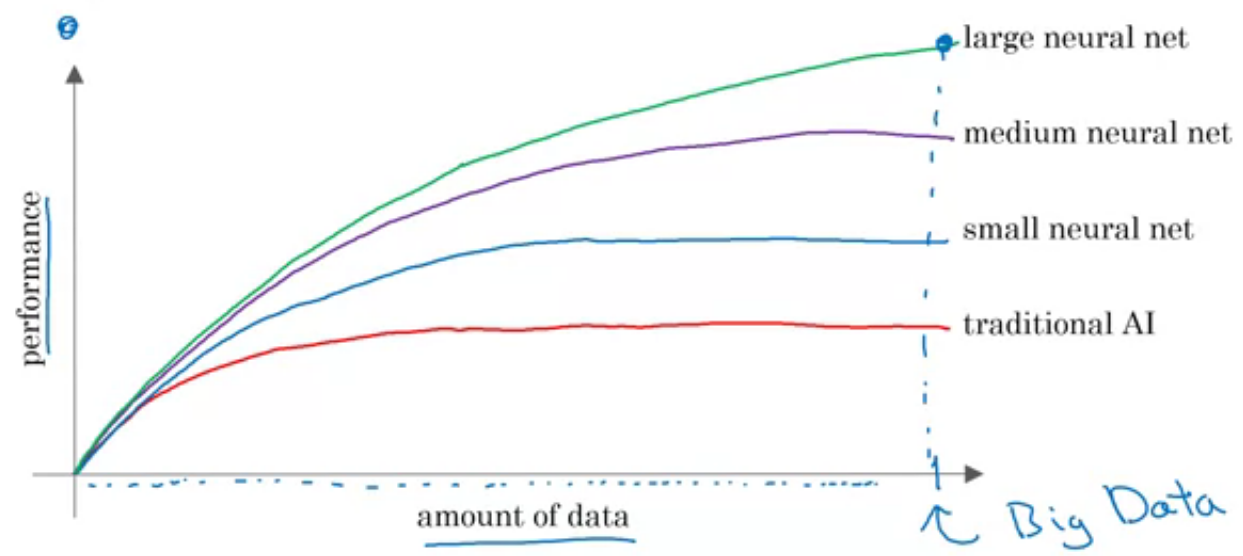
\includegraphics[scale=.25]{big-data}
		\caption{Large neural net + Big Data = High Performance \citep{ng2019AIForEveryone}}
		\label{fig:big-data}
	\end{figure}
\end{frame}

\section{What is Data?}
\begin{frame}{Example of a Table of Data (Dataset) (1/3)}
	\begin{table}[!ht]
		\centering
		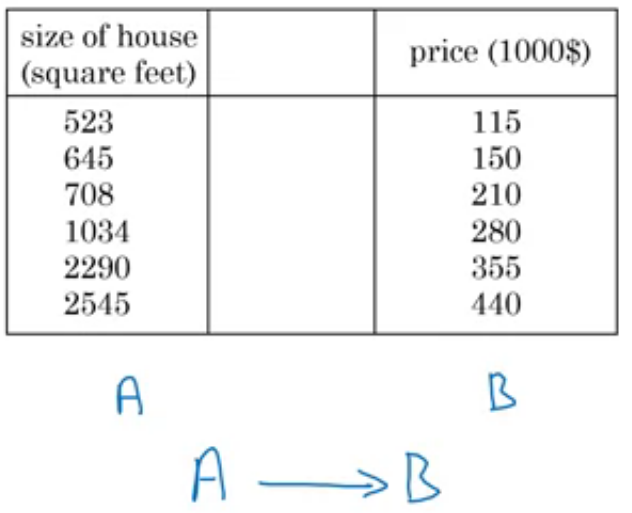
\includegraphics[scale=.3]{example-dataset-2}
		\caption{House prices dataset~\citep{ng2019AIForEveryone}}
		\label{fig:example-dataset-2}
	\end{table}
\end{frame}


\begin{frame}{Example of a Table of Data (Dataset) (2/3)}
	\begin{table}[!ht]
		\centering
		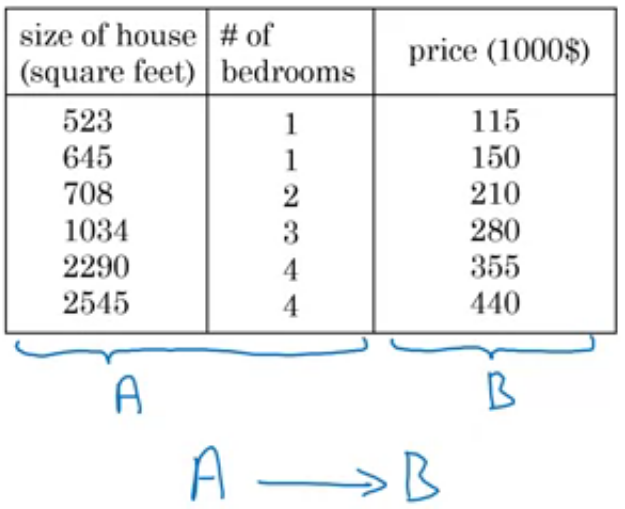
\includegraphics[scale=.3]{example-dataset-1}
		\caption{House prices dataset~\citep{ng2019AIForEveryone}}
		\label{fig:example-dataset-1}
	\end{table}
\end{frame}

\begin{frame}{Example of a Table of Data (Dataset) (3/3)}
	\begin{table}[!ht]
		\centering
		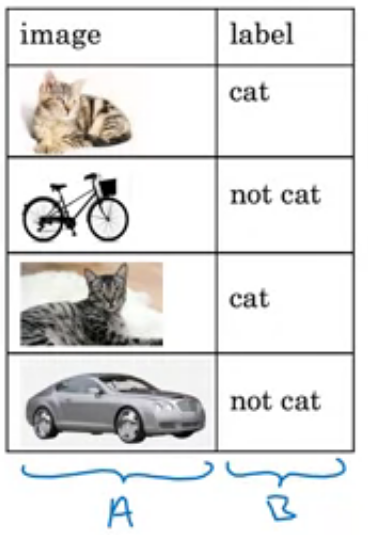
\includegraphics[scale=.3]{example-dataset-3}
		\caption{Cat images dataset~\citep{ng2019AIForEveryone}}
		\label{fig:example-dataset-3}
	\end{table}
\end{frame}

\begin{frame}{Acquiring data}
	\begin{itemize}
		\item<2-> Manual labeling
		\begin{center}
			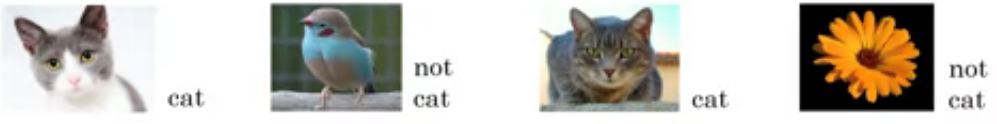
\includegraphics[scale=.3]{manual-labeling}
		\end{center}
		\item<3-> From observing behaviors
		\begin{center}
			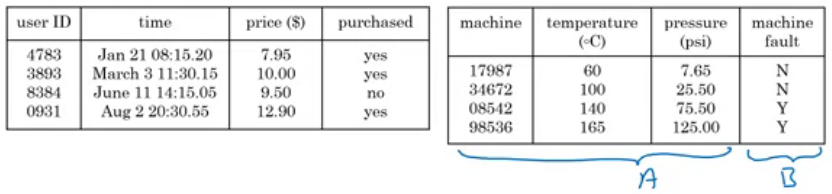
\includegraphics[scale=.35]{observing-behaviors}
		\end{center}
		\item<4-> Download from websites / partnerships \\
		Contoh: \href{https://www.kaggle.com/datasets}{\textcolor{orange}{\underline{ Kaggle}}}, \href{http://archive.ics.uci.edu/ml/datasets.php}{\textcolor{blue}{\underline{UCI Machine Learning Repo}}}		
	\end{itemize}
\end{frame}

\begin{frame}{Data is Messy}
	\begin{itemize}
		\item<2-> Garbage in, garbage out
		\item<3-> Data problems: \textit{incorrect labels} and \textit{missing values} 
		\begin{center}
			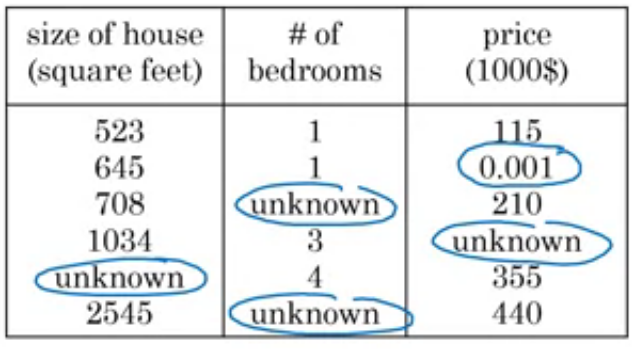
\includegraphics[scale=.3]{data-problems} 
		\end{center}
		\item<4-> Multiple types of data \\
		\textit{images}, \textit{audio}, \textit{text} $\Rightarrow$ \textbf{unstructured data}					
	\end{itemize}
\end{frame}

\section{Machine Learning vs. Data Science}
\begin{frame}{AI, Machine Learning, and Data Science}
	\begin{figure}[!ht]
		\centering
		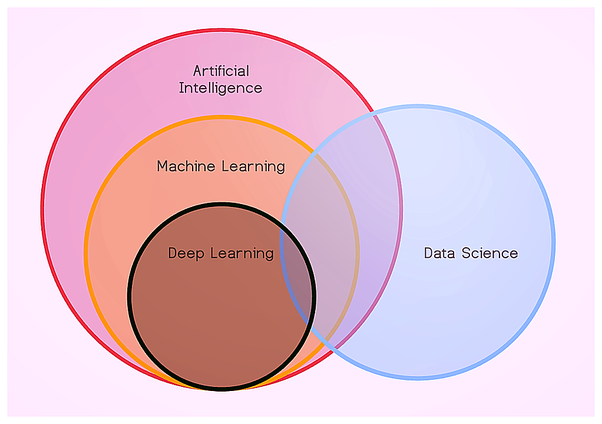
\includegraphics[scale=.45]{diagram-venn-deep-learning}
		\caption{Relationship among AI, ML, DL, and DS~\citep{kharkovyna2019ABeginnersGuide}}
	\end{figure}
\end{frame}

\begin{frame}{Machine Learning vs. Data Science (1/2)}
	\begin{figure}[!ht]
		\centering
		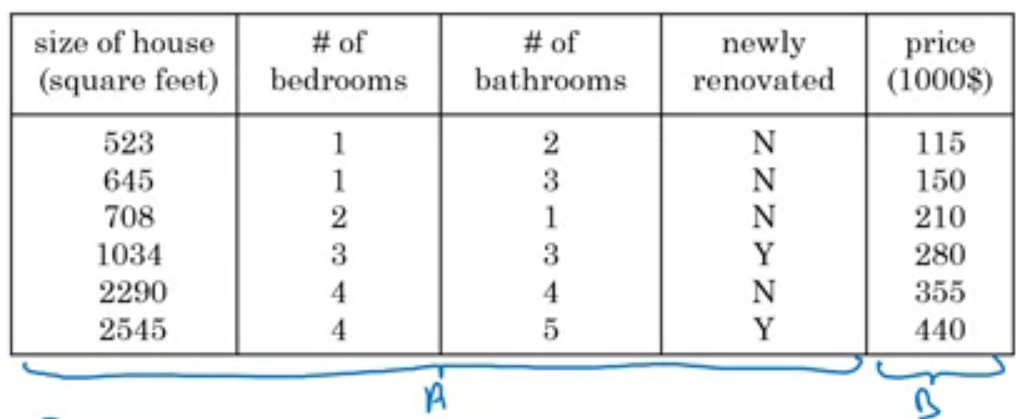
\includegraphics[scale=.25]{ml-vs-ds}		
		\caption{Home prices~\citep{ng2019AIForEveryone}}
	\end{figure}
	\begin{itemize}
		\item<2-> \textbf{According to \textit{Machine Learning}}: \\
	$A \longrightarrow B$: Running AI system (e.g., websites / mobile app)
		\item<3-> 	\textbf{According to \textit{Data Science}}: \\
	\textit{Homes with 3 bedrooms are more expensive than homes with 2 bedrooms of a similar size}. \\		
	\textit{Newly renovated homes have a 15\% premium}.		
	\end{itemize}
%	\vspace*{-.5cm}			
\end{frame}

\begin{frame}{Machine Learning vs. Data Science (2/2)}
	\begin{table}[!ht]
		\centering
		\begin{tabular}{cc}
			\textbf{Machine Learning}        & \textbf{Data Science} \\
			                                 &                       \\
			 \onslide<2-> "\textit{Field of study that gives}      & \onslide<3-> \textit{Science of extracting knowledge} \\
			 \onslide<2-> \textit{computers the ability to learn}   & \onslide<3-> \textit{and insights from data.} \\
			 \onslide<2-> \textit{without being explicitly}         &   \\
			 \onslide<2-> \textit{programmed.}"                     &   \\
			 \onslide<2-> $\longrightarrow$ \textbf{software}       & \onslide<3-> $\longrightarrow$ \textbf{slide presentation} or \textbf{report}  \\
			 \onslide<2-> -Arthur Samuel (1959)           & 
		\end{tabular}
	\end{table}
\end{frame}

\section{Deep Learning}
\begin{frame}{Dataset: Home Prices}
		\begin{figure}[!ht]
		\centering
		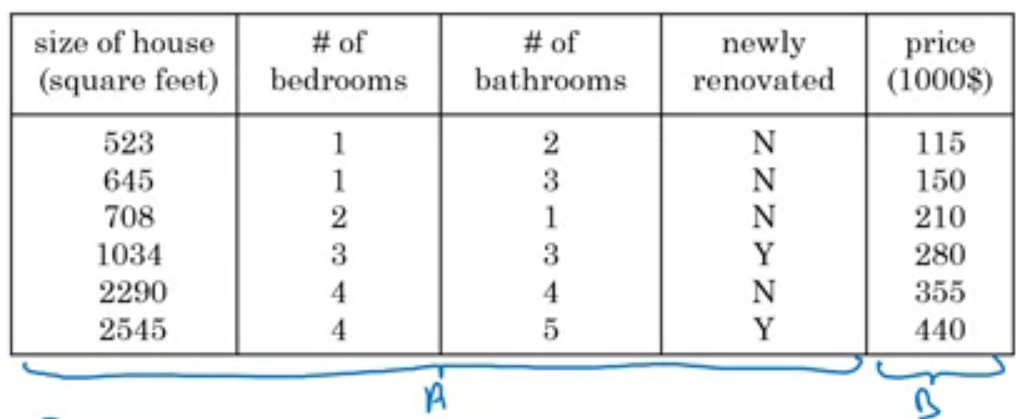
\includegraphics[scale=.25]{ml-vs-ds}		
		\caption{Home prices~\citep{ng2019AIForEveryone}}
	\end{figure}
\end{frame}

\begin{frame}{Deep Learning (1/3)}
	\begin{center}
		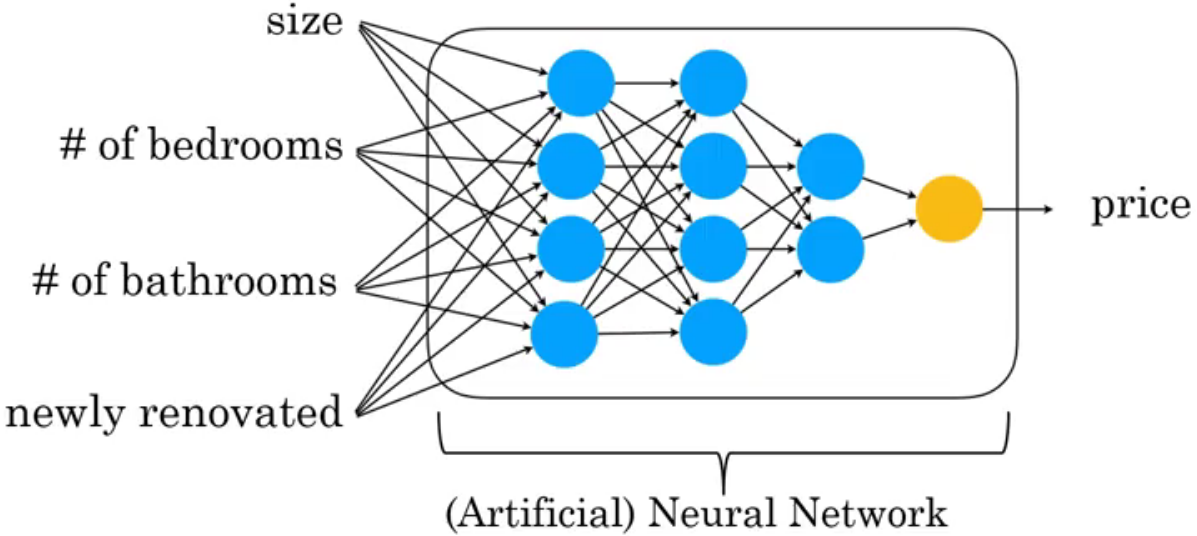
\includegraphics[scale=.275]{deep-learning}
	\end{center}	
\end{frame}

\begin{frame}{Deep Learning (2/3)}
		\begin{figure}[!ht]
	\centering
	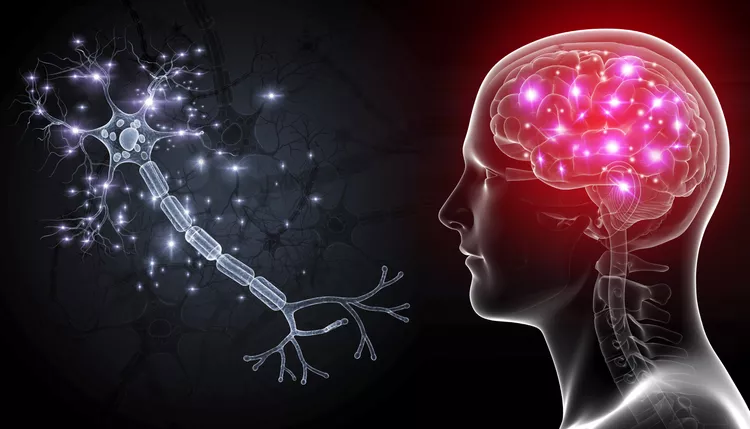
\includegraphics[scale=.4]{images/brain-neurons}		
	\caption{Neuron-neuron di Otak \citep{ankrom2020howbrain}}
\end{figure}
\end{frame}

\begin{frame}{Deep Learning (2/3)}
	\begin{center}
		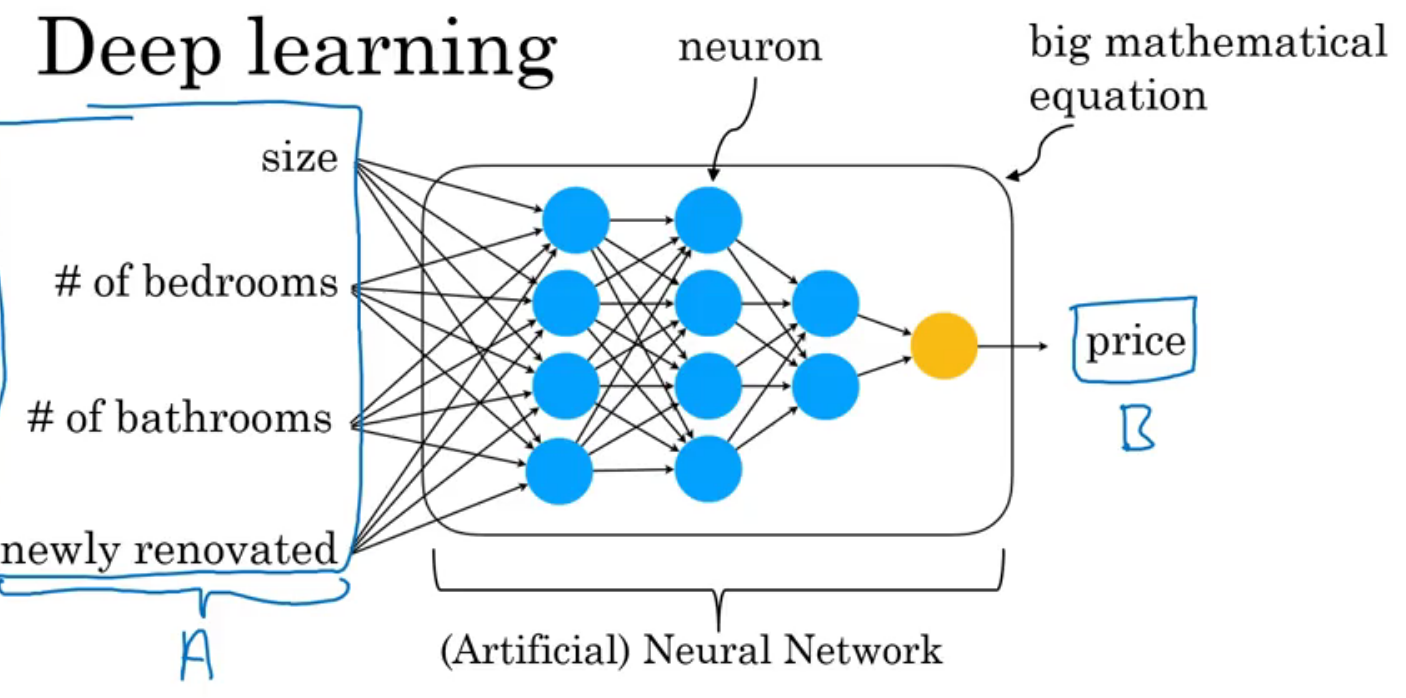
\includegraphics[scale=.24]{deep-learning-2}
	\end{center}	
\end{frame}

\section{Non-technical explanation of deep learning}
\begin{frame}{Demand prediction (1/2)}
	\begin{columns}[c]		
		\begin{column}{0.6\textwidth}
			\hspace{20pt}
			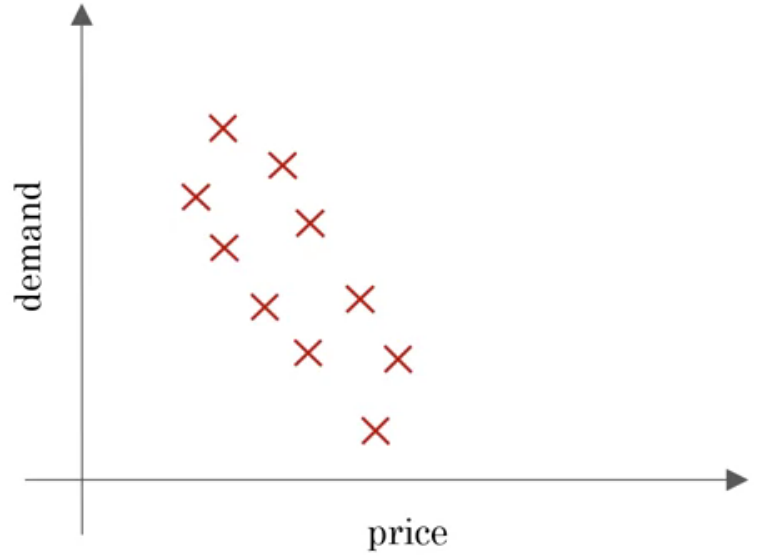
\includegraphics[scale=.225]{demand-prediction}
		\end{column}
		\hspace{-10pt}
		\begin{column}{0.4\textwidth}
			
\includegraphics[scale=.225]{t-shirt}				
		\end{column}		
	\end{columns}	
\end{frame}

\begin{frame}{Demand prediction (2/2)}
	\centering
	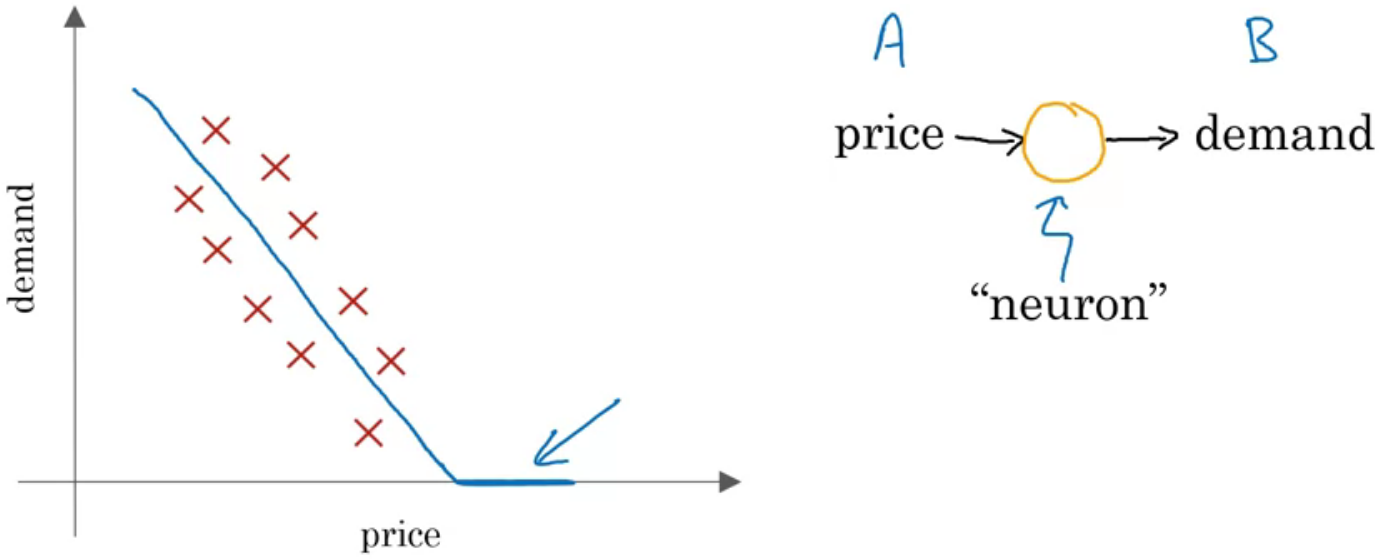
\includegraphics[scale=.225]{demand-prediction-line}
\end{frame}

\begin{frame}{Demand prediction: a little bit more complex (1/4)}
	\centering
	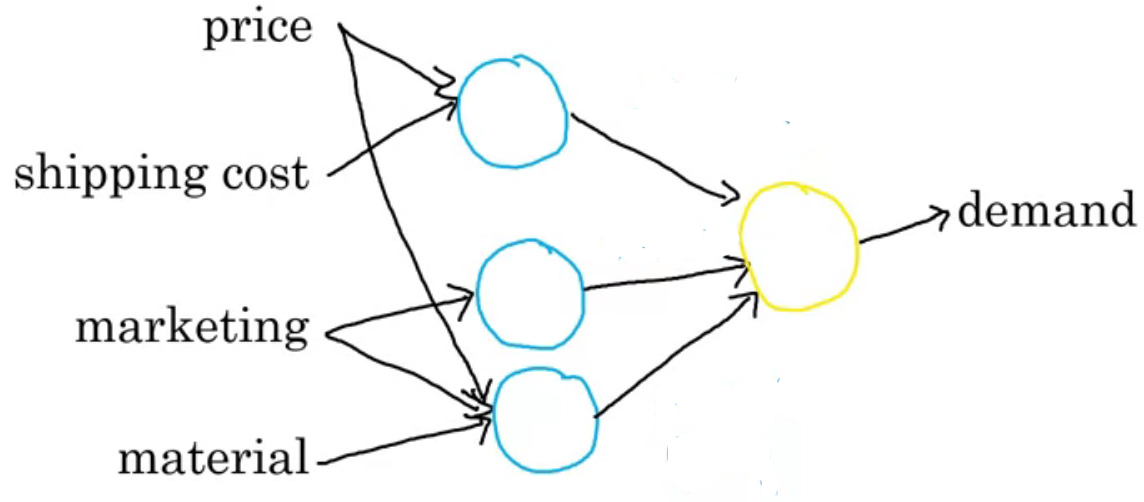
\includegraphics[scale=.275]{demand-prediction-nn-0.png}
\end{frame}

\begin{frame}{Demand prediction: a little bit more complex (2/4)}
	\centering
	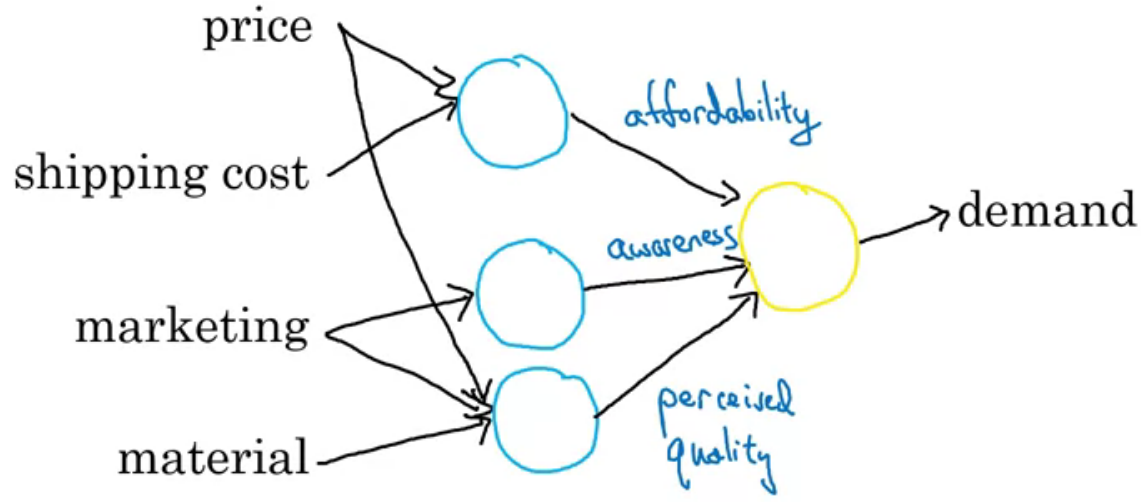
\includegraphics[scale=.275]{demand-prediction-nn.png}
\end{frame}



\begin{frame}{Demand prediction: a little bit more complex (3/4)}
	\centering
	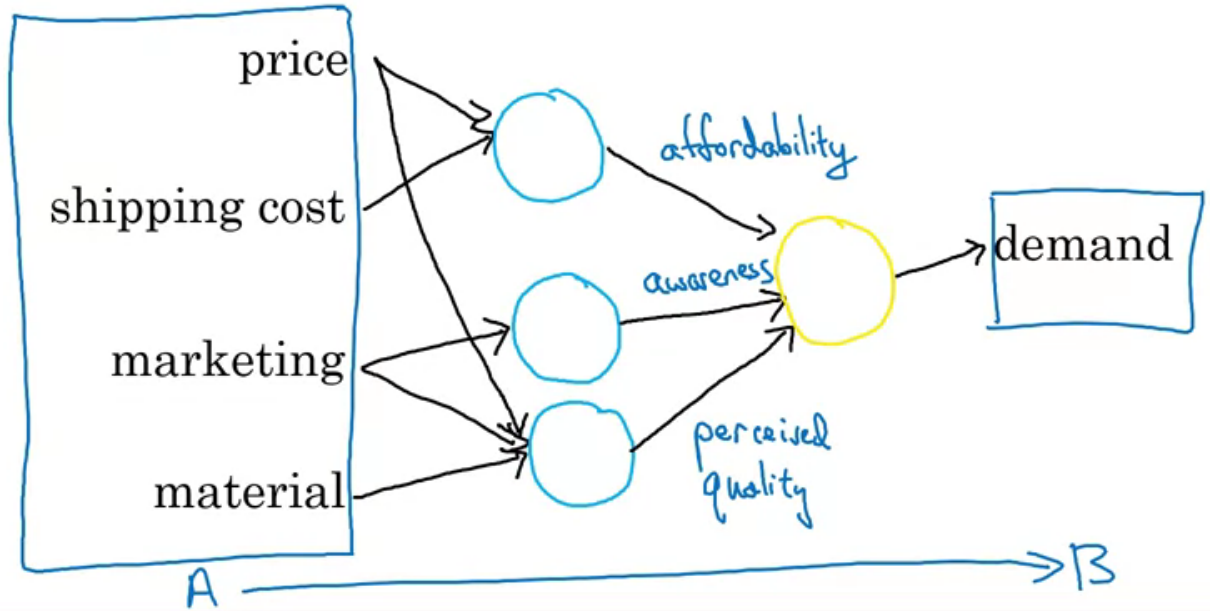
\includegraphics[scale=.275]{demand-prediction-nn-2.png}
\end{frame}

\begin{frame}{Demand prediction: a little bit more complex (4/4)}
	\centering
	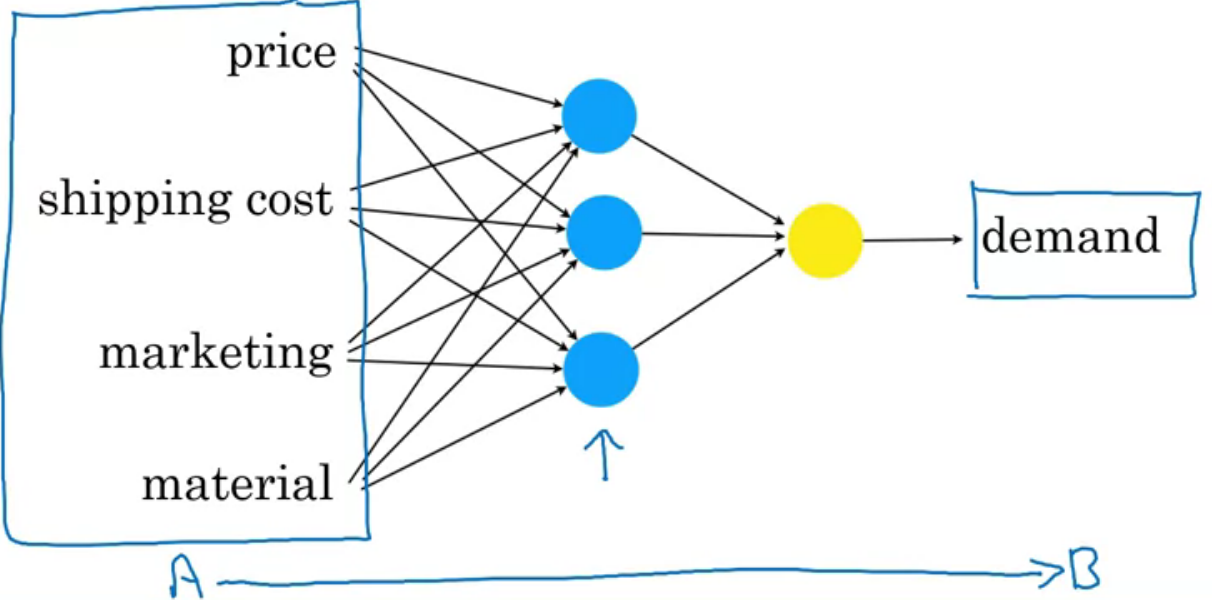
\includegraphics[scale=.275]{demand-prediction-nn-3.png}
\end{frame}


\begin{frame}{NN Application: Face recognition (1/3)}
	We want to build a system that recognizes people from pictures.
	\begin{figure}[!ht]
		\centering
		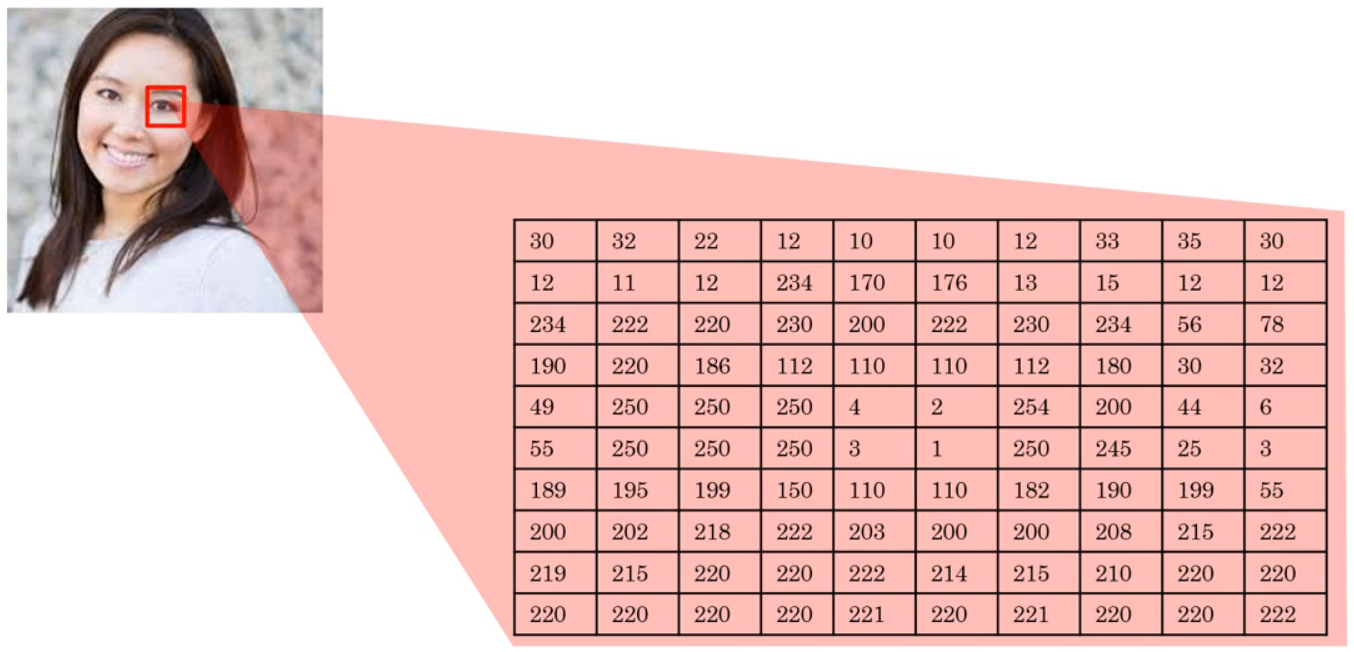
\includegraphics[scale=.25]{face-recognition-intro}
		\caption{What a computer sees from an image (assume the picture is grayscale)~\citep{ng2019AIForEveryone}}
	\end{figure}
	
\end{frame}

\begin{frame}{NN Application: Face recognition (2/3)}
		\centering
		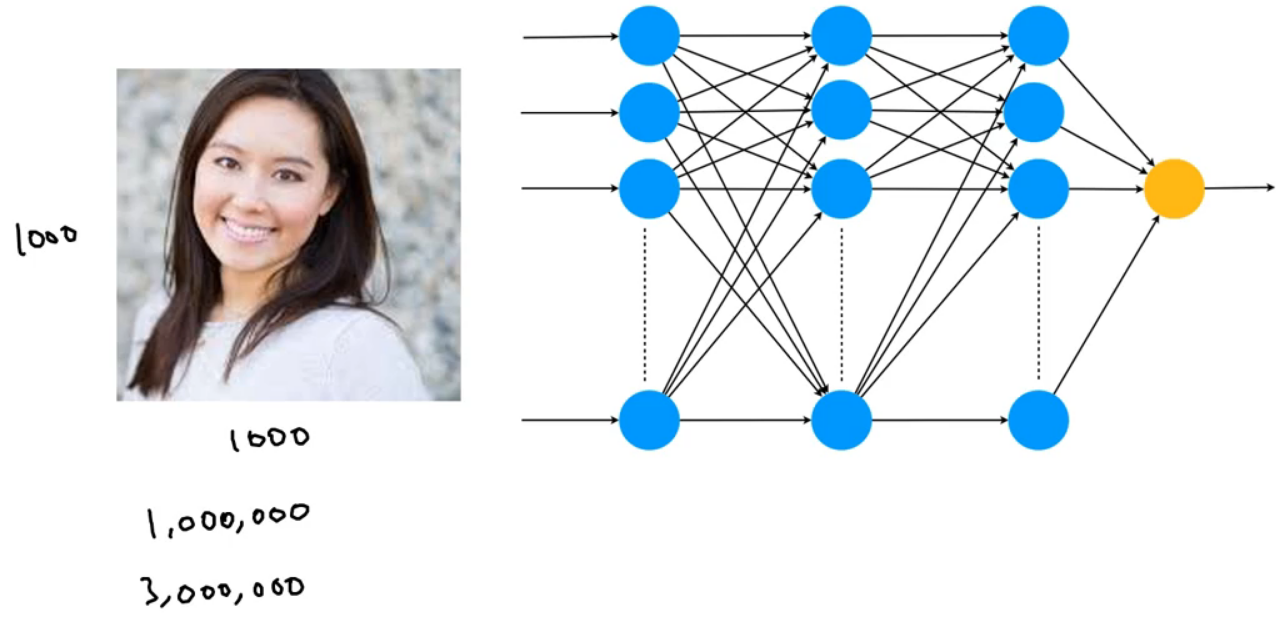
\includegraphics[scale=.25]{face-recognition-intro-2}
\end{frame}

\begin{frame}{NN Application: Face recognition (3/3)}
		\centering
		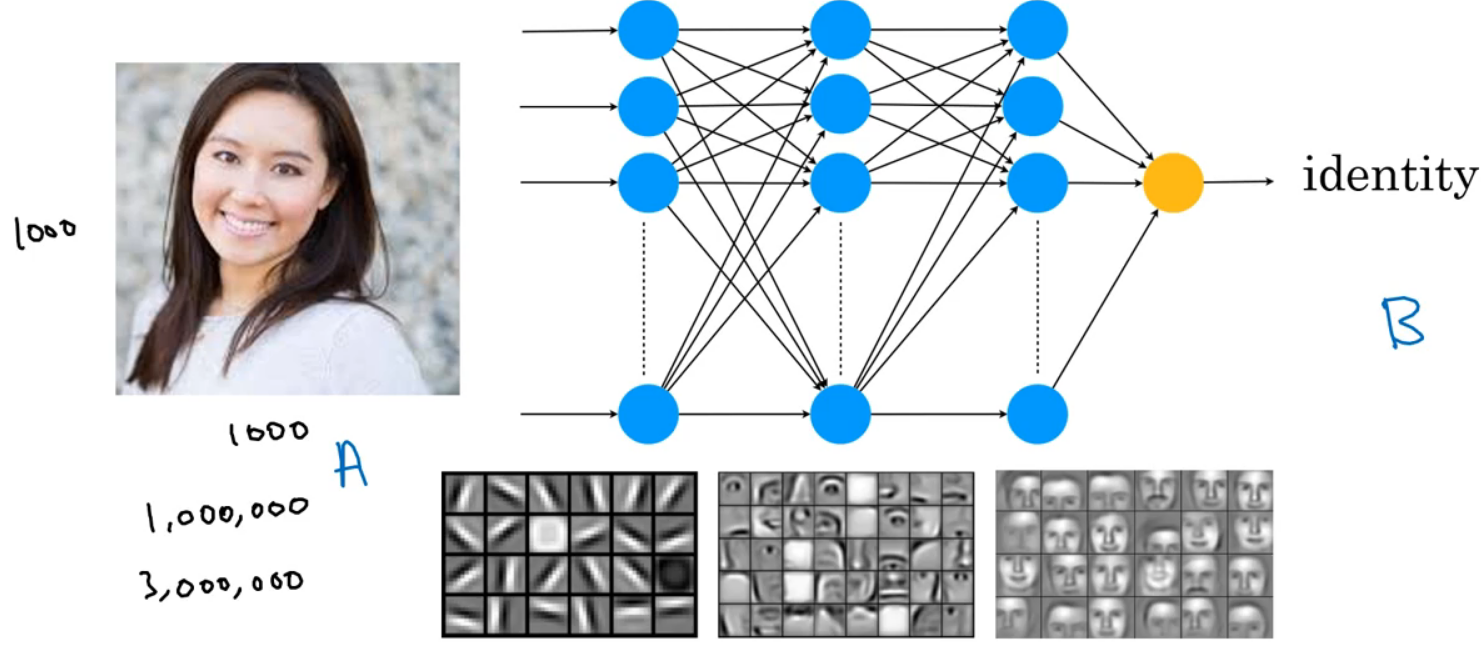
\includegraphics[scale=.225]{face-recognition-intro-3}
\end{frame}

\begin{frame}{How Does a Neural Network Learn?}
	Watch \href{https://phiresky.github.io/neural-network-demo/}{\textcolor{pink}{\textbf{a Demo}}} by~\citet{phiresky2017neuralnetwork}.
\end{frame}


\section{What Machine Learning Can and Cannot Do}
\begin{frame}{Supervised Learning}
	\begin{center}
		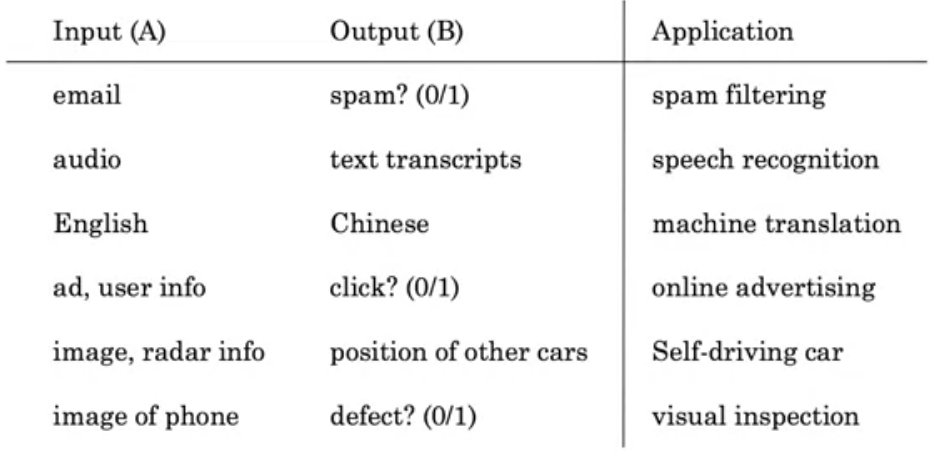
\includegraphics[scale=.3]{what-ML-can-do}
	\end{center}
	\begin{center}
		\pause \textit{Anything you can do with 1 second of thought, we can probably now or soon automate.}
	\end{center}
\end{frame}

\begin{frame}{What machine learning today can and cannot do}
	You ordered a toy. The toy arrived late. Therefore, you write an email:
	
	\bigskip
	\textit{The toy arrived two days late, so I wasn't able to give it to my niece for her birthday.} \\
	\textit{Can I return it?}

	\bigskip
	\pause \textbf{Machine Learning Can Do}: \\
	$\longrightarrow$ "\textit{Refund request}" \\
	Input text $\longrightarrow$ Refund/Shipping/Other \\
	$A \longrightarrow B$
	
	\bigskip
	\pause \textbf{Machine Learning Cannot Do Elegantly Yet}: \\
	$\longrightarrow$ "\textit{Oh, sorry to hear that. I hope your niece had a good birthday. Yes, we can help with ...}"	
	
\end{frame}

\begin{frame}{What happens if you try?}
	\begin{tabular}{lcl}
		\textbf{Input (A)} & $\longrightarrow$ & \textbf{Output (B)} \\
		User email	       &                   & 2-3 paragraph response
	\end{tabular}

	\bigskip
	
	\textbf{Train Data}: 1000 examples 
	
	\bigskip
	
	\begin{tabular}{lcl}
		\onslide<2-> "My box was damaged" & $\longrightarrow$ & Thank you for your email. \\
		   	                 &                     &   \\
		\onslide<3-> "Where do I write a review?" & $\longrightarrow$ & Thank you for your email. \\		   	                 
		   	                 &                     &   \\
		\onslide<4-> "What's the return policy" & $\longrightarrow$ & Thank you for your email. \\		   	                 		   	                 		   	                 &                     &   \\
		\onslide<5-> "When is my box arriving?" & $\longrightarrow$ & Thank yes now your....
	\end{tabular}
\end{frame}
	
\begin{frame}{What makes an ML problem easier}
	\begin{enumerate}
		\item<2-> Learning a "simple" concept \\
		\begin{center}
			
			\scalebox{2}{
				$\leq 1 \text{ sec}$
			} 							
		\end{center}		
		
		\bigskip		
		
		\item<3-> Lots of data available \\
		\begin{center}
			
			\scalebox{2}{
				$A \longrightarrow B$
			} \\	
			\scalebox{1}{
				\qquad input \qquad \; \; output
			}							
		\end{center}				
	\end{enumerate}
\end{frame}	

\section{More examples of what ML can and cannot do}
\begin{frame}{Self-driving car}
	\begin{columns}[c]		
		\begin{column}{0.5\textwidth}
			\includegraphics<2->[scale=.225]{kiri-can}
			\vspace*{1.75cm}
		\end{column}
		\hspace{-50pt}
		\vrule{}
		\begin{column}{0.5\textwidth}
			\includegraphics<3->[scale=.225]{kanan-can}				
	\begin{enumerate}
		\item<4-> Data 
		\item<5-> Need high accuracy
	\end{enumerate}					
		\end{column}		
	\end{columns}	
\end{frame}
	
\begin{frame}{X-ray diagnosis}
	\begin{center}
		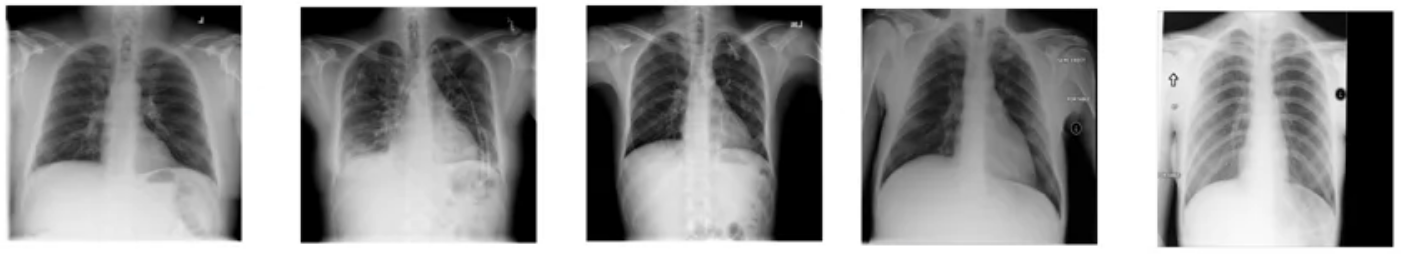
\includegraphics[scale=.225]{x-ray}	
	\end{center}		
	\centering
	\begin{tabular}{l|l}
		\multicolumn{1}{c|}{\textbf{Can do}} & \multicolumn{1}{c}{\textbf{Cannot do}} \\
		                                                 &   \\
	    \onslide<2->Diagnose pneumonia from                      &  \onslide<3->  Diagnose pneumonia from \\
	    \onslide<2->$\thicksim$10,000 labeled images             &  \onslide<3->  10 images of medical textbook \\
	                                                 &    \onslide<3->chapter explaining pneumonia	                  
	\end{tabular}	
\end{frame}

\begin{frame}{Strengths and weaknesses of machine learning}
	ML tends to work well when:
	\begin{enumerate}
		\item<2-> Learning a "simple" concept 
		\item<3-> There are lots of data available
	\end{enumerate}
	
	\bigskip	
	
	ML tends to work poorly when:
	\begin{enumerate}
		\item<4-> Learning complex concepts from small amounts of data
		\item<5-> It is asked to perform on new types of data
	\end{enumerate}
	\begin{center}
		\includegraphics<5->[scale=.275]{new-types-of-data}
	\end{center}
\end{frame}

\begin{frame}{Machine Learning}	
	The way a machine or computer learns can be categorized into several types~\citep{geron2019handson}:
	\begin{itemize}
		\item<2-> Supervised Learning,
		\item<3-> \textcolor <4-> {orange} {\textbf<4->{Unsupervised Learning}}.
	\end{itemize}	
	
\end{frame}

\begin{frame}{Unsupervised learning (1/2)}
	Clustering potato chip sales
	\begin{center}
		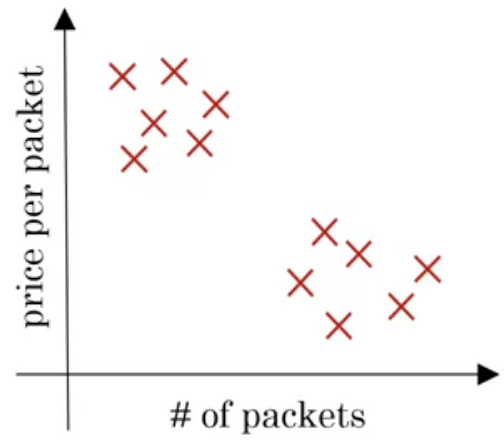
\includegraphics[scale=.25]{potato-chip-sales} \qquad \includegraphics<2->[scale=.25]{potato-chip-sales-2}
	\end{center}
	
\end{frame}

\begin{frame}{Unsupervised learning (2/2)}
	\textbf{Unsupervised learning}:
	\begin{center}
		\textit{Given data (without any specific desired output labels), find something interesting about the data.}
	\end{center}
	
	\textbf{Another example of unsupervised learning:}
	
	\bigskip	
	
	\pause Finding cats from unlabeled YouTube videos
	\begin{center}
		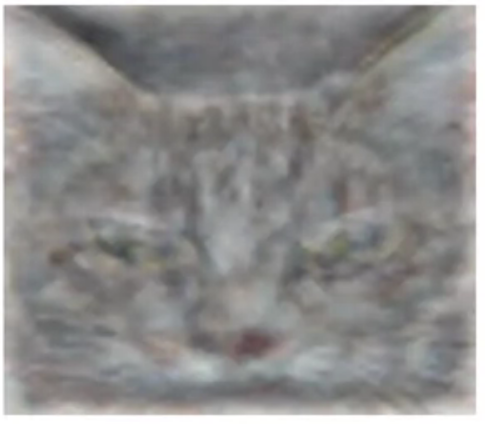
\includegraphics[scale=.25]{google-cats}
	\end{center}	
\end{frame}

\section{Jalur Peminatan AI: Becoming AI Specialist}
\begin{frame}{Computer Vision (1/7)}
	\begin{itemize}
		\item Image classification/Object recognition 
		\begin{center}
			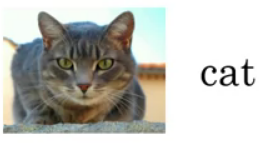
\includegraphics[scale=.4]{image-classification}	
		\end{center}
	\end{itemize}
\end{frame}

\begin{frame}{Computer Vision (2/7)}
	\begin{itemize}
		\item Face verification \& face identification
	\end{itemize}	
	\begin{figure}[!ht]
	\centering
	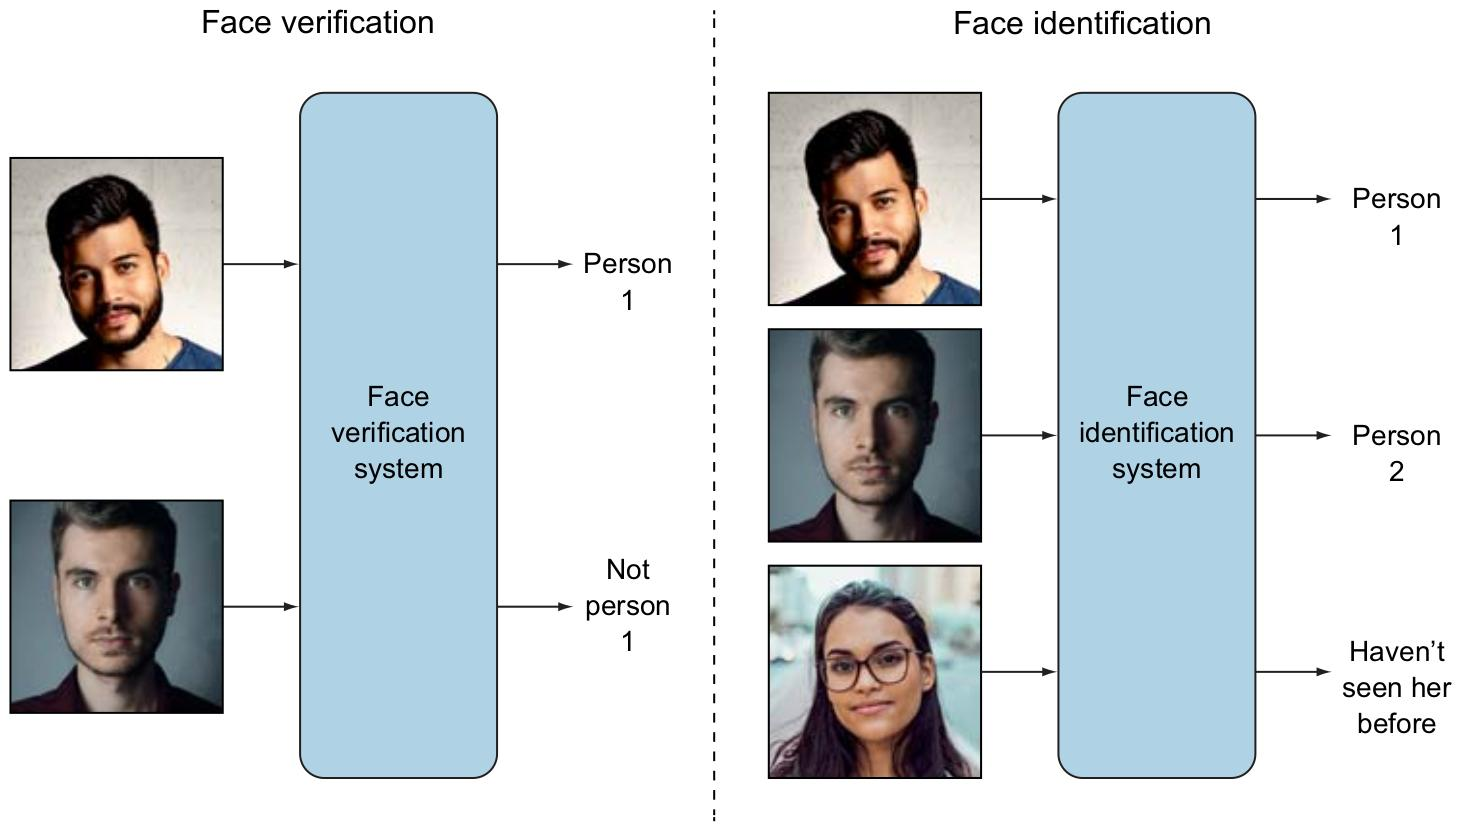
\includegraphics[scale=.232]{images/face-identification-recognition.jpg}
	\caption{Example of face verification (left) and face recognition (right) \citep{elgendy2020deeplearning4vision}}
\end{figure}
\end{frame}

\begin{frame}{Computer Vision (3/7)}
	\begin{itemize}
		\item Object detection
		\begin{center}
			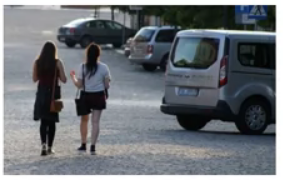
\includegraphics[scale=.4]{object-detection-1} \qquad \includegraphics<2->[scale=.4]{object-detection-2}
			\bigskip			
			\includegraphics<3->[scale=.4]{object-detection-3}	
		\end{center}
	\end{itemize}
\end{frame}

\begin{frame}{Computer Vision (4/7)}
	\begin{itemize}
		\item Image Segmentation
		\begin{center}
			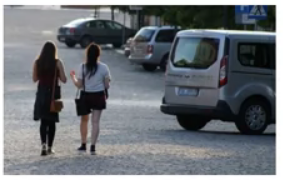
\includegraphics[scale=.4]{object-detection-1} \qquad \includegraphics<2->[scale=.4]{image-segmentation}	
		\end{center}
		\item<3-> Tracking
		\begin{center}
			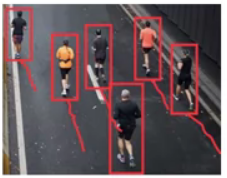
\includegraphics[scale=.4]{tracking}
		\end{center}
	\end{itemize}
\end{frame}

\begin{frame}{Computer Vision (5/7)}
	\begin{itemize}
		\item Membuat gambar baru dari style pelukis ternama.
	\end{itemize}	
\begin{figure}[!ht]
	\centering
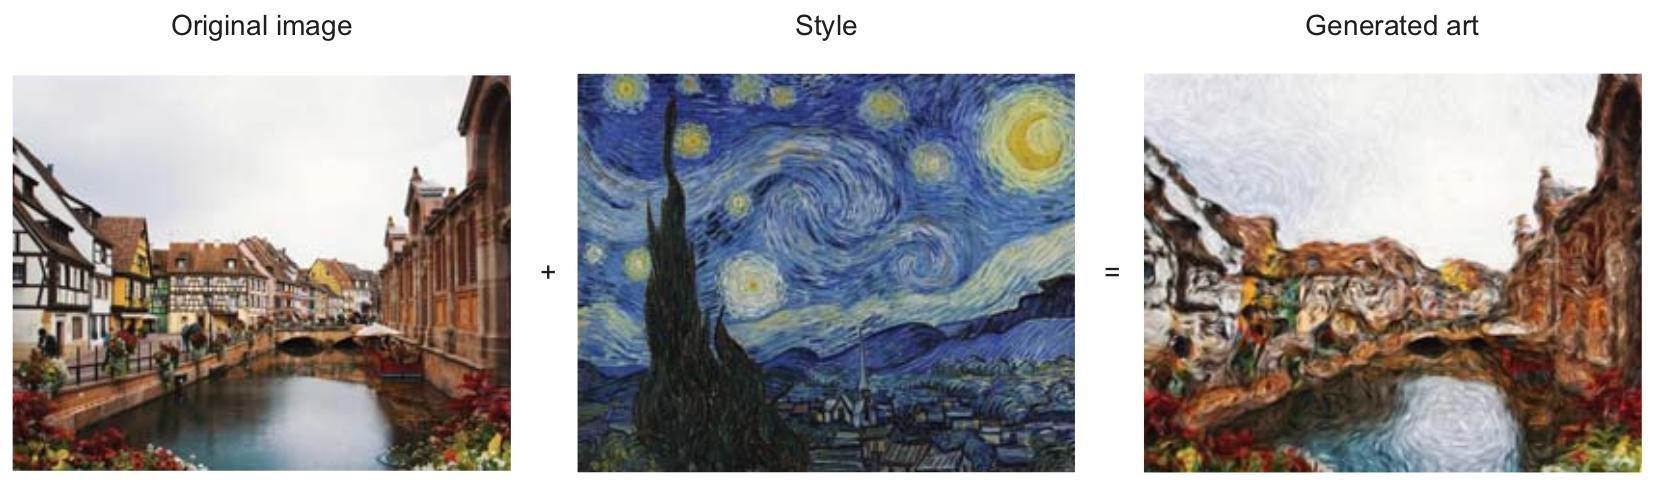
\includegraphics[scale=.2]{images/generating-style}
\caption{Style transfer from Van Goghs The Starry Night onto the original image \citep{elgendy2020deeplearning4vision}}
\end{figure}		
\end{frame}

\begin{frame}{Computer Vision (6/7)}
	\begin{itemize}
		\item Membuat gambar baru dari deskripsi teks
	\end{itemize}
	\begin{figure}[!ht]
	\centering
	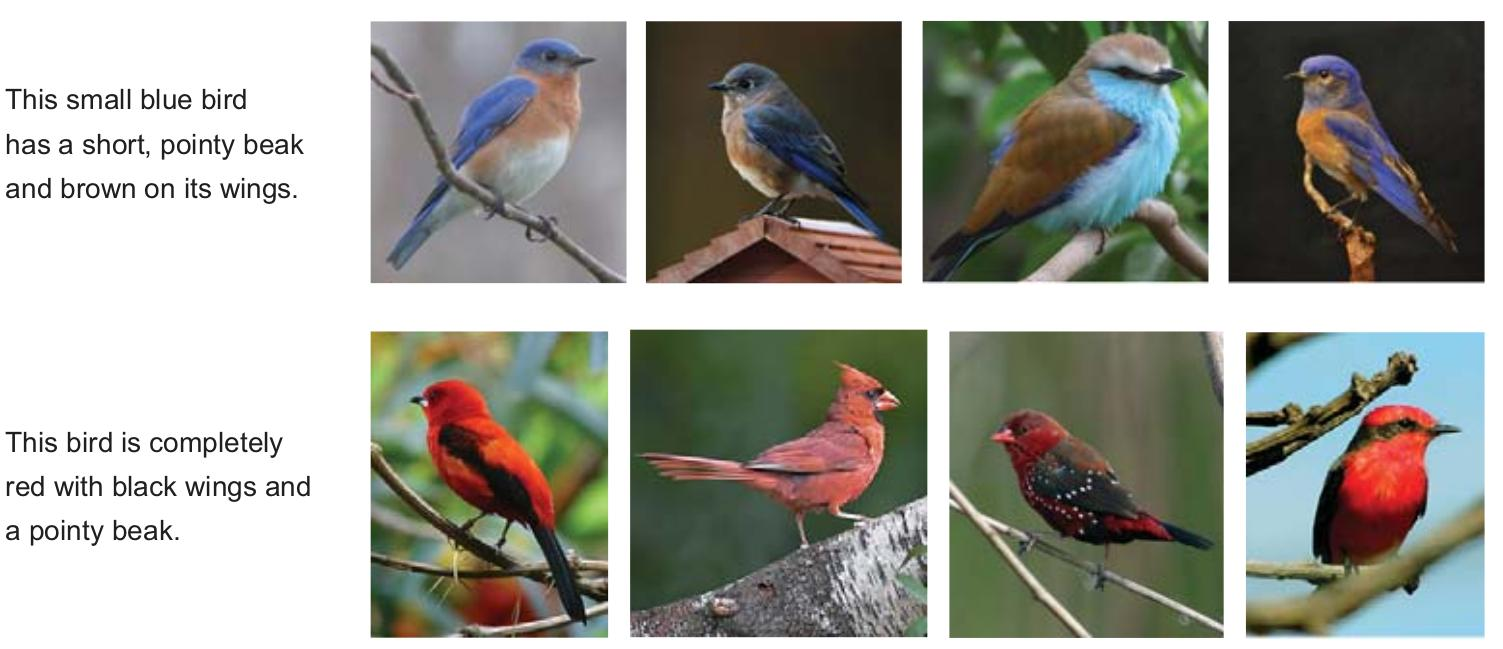
\includegraphics[scale=.225]{images/gans+text+cv.jpg}
	\caption{StackGAN use a textual description of an object to generate a high-resolution image of the object matching that description \citep{elgendy2020deeplearning4vision}}
\end{figure}		
\end{frame}

\begin{frame}{Computer Vision (7/7)}
	\begin{itemize}
	\item Image recommendation system
\end{itemize}
\begin{figure}[!ht]
	\centering
	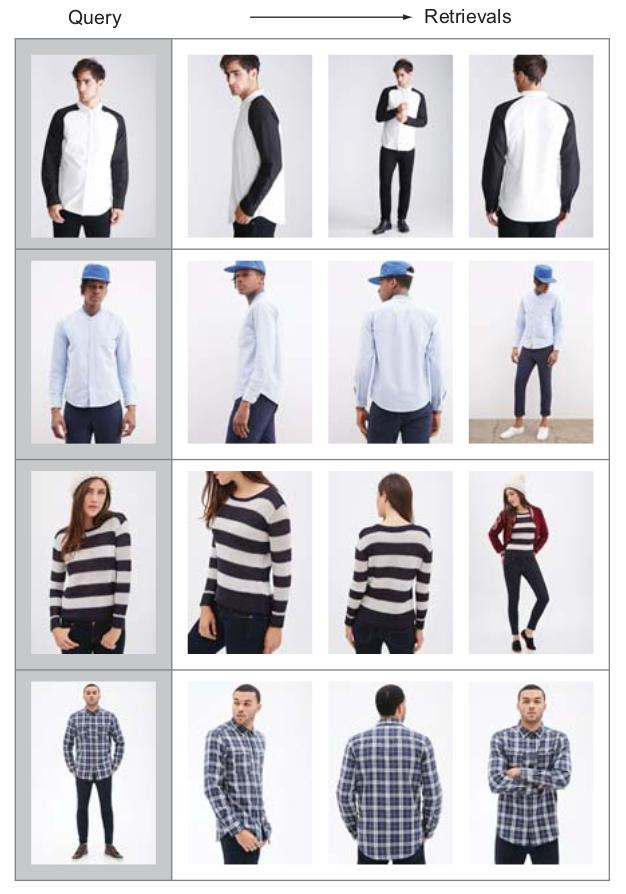
\includegraphics[scale=.225]{images/image-recommendation.jpg}
	\caption{Apparel search \citep{elgendy2020deeplearning4vision}}
\end{figure}		
\end{frame}

\begin{frame}{Natural Language Processing (1/8)}
	\begin{itemize}		
		\item Information search atau information retrieval \citep{kochmar2022getting}
	\end{itemize}
	\textbf{Contoh 1:}
	\begin{center}
		
\includegraphics[scale=.25]{images/search-engine-1}
	\end{center}
	\textbf{Contoh 2:}
	\begin{center}
		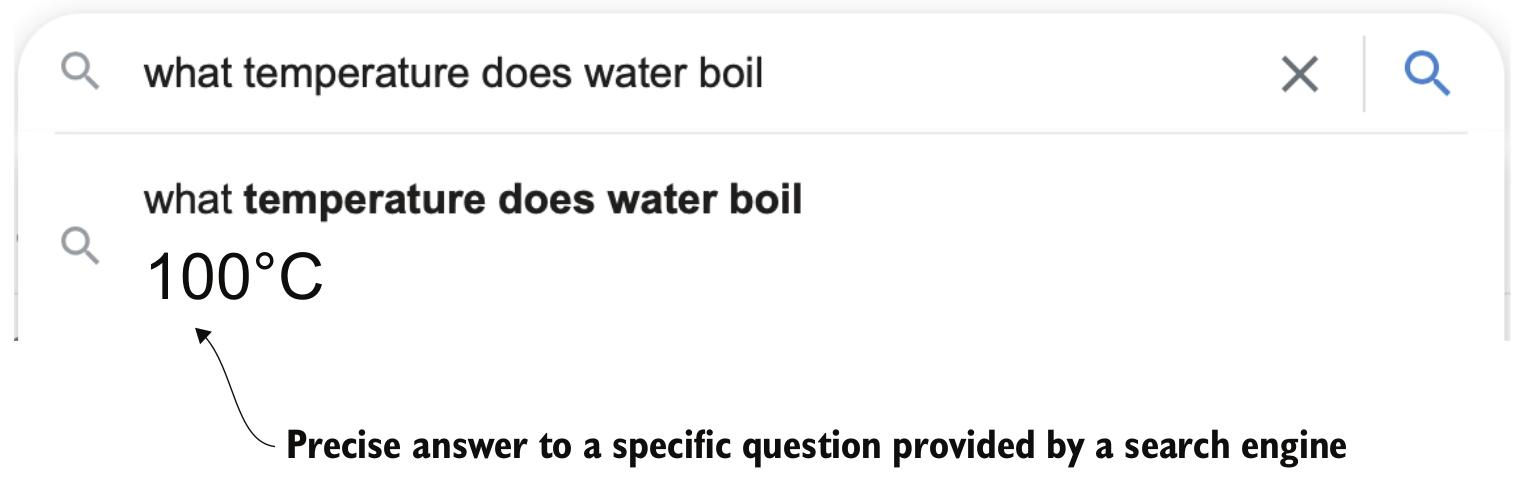
\includegraphics[scale=.2]{images/search-engine-2}
	\end{center}
\end{frame}

\begin{frame}{Natural Language Processing (2/8)}
	\begin{itemize}		
		\item Advanced information search: Asking the machine precise questions
	\end{itemize}
	\begin{center}
		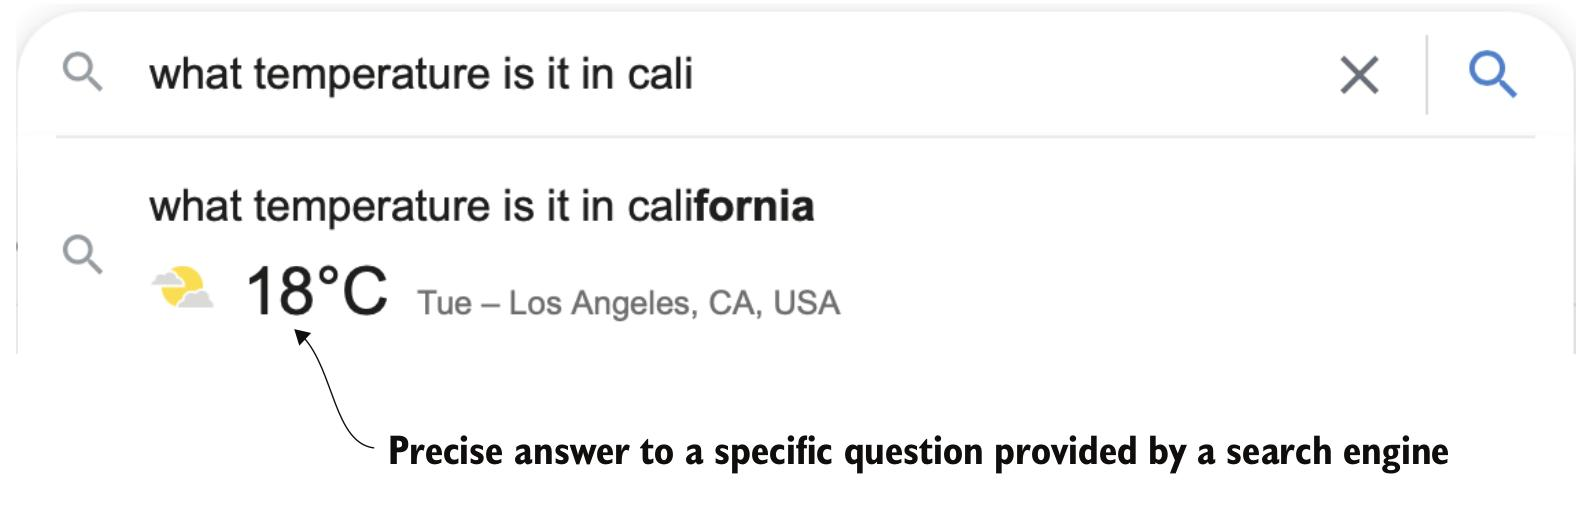
\includegraphics[scale=.225]{images/search-engine-3}
	\end{center}
\end{frame}

\begin{frame}{Natural Language Processing (3/8)}
The search for factual information on Google returns both the precise answer to the question and the accompanying explanation.
	\begin{center}
		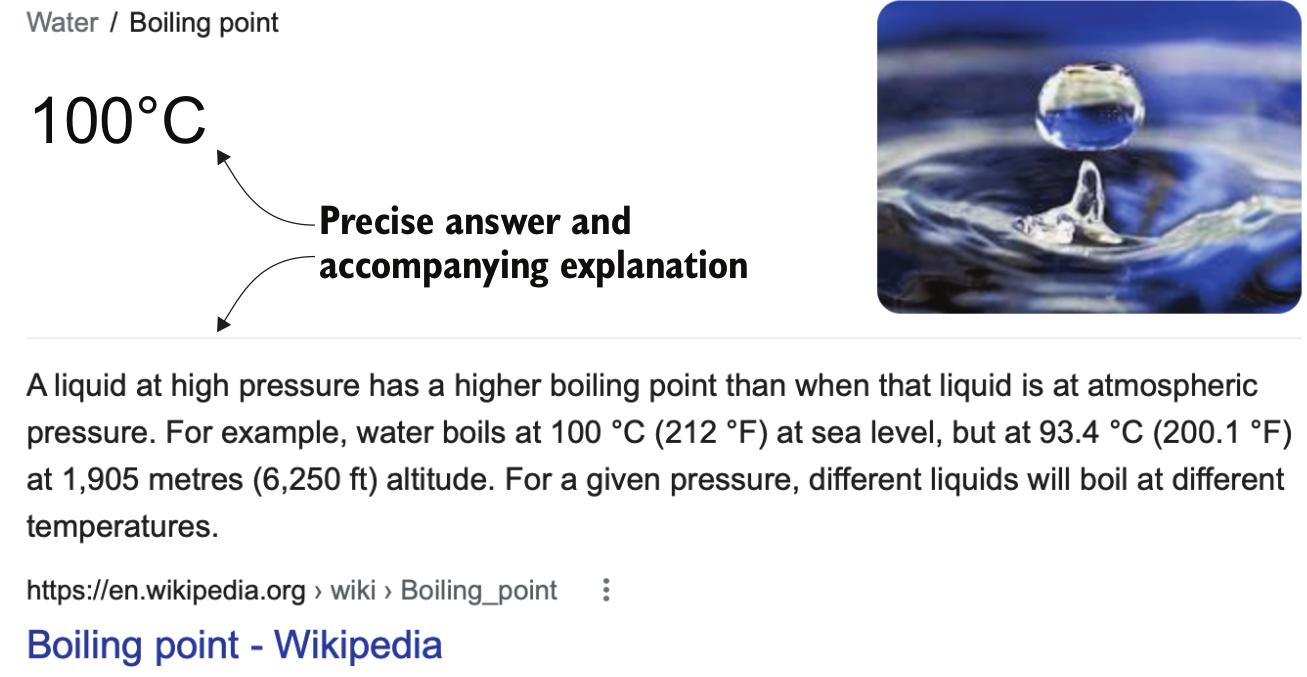
\includegraphics[scale=.25]{images/search-engine-4}
	\end{center}
\end{frame}

\begin{frame}{Natural Language Processing (4/8)}
	\begin{itemize}
		\item Conversational agents dan intelligent virtual assistants
	\end{itemize}
	\begin{center}
		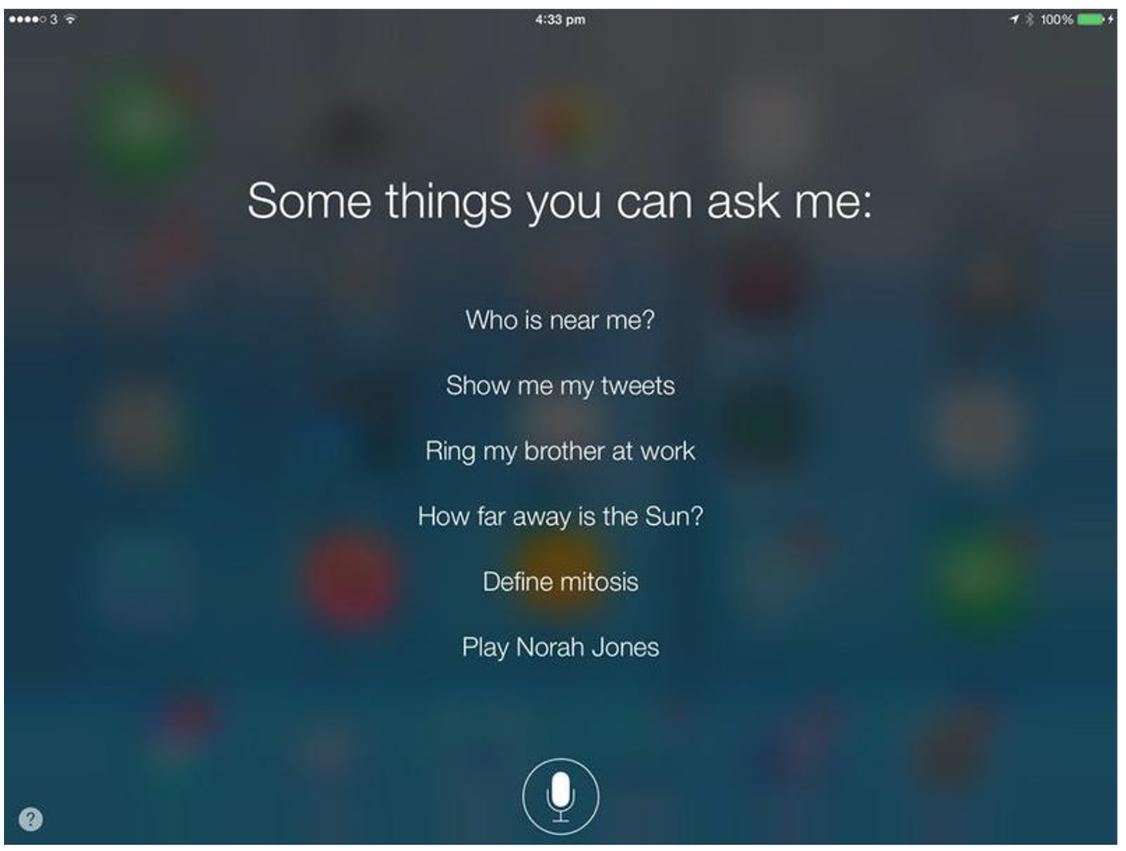
\includegraphics[scale=.225]{images/conversational-1}
	\end{center}
\end{frame}

\begin{frame}{Natural Language Processing (5/8)}
	\begin{itemize}
		\item Text prediction dan language generation
	\end{itemize}
	\begin{figure}[!ht]
		\centering
		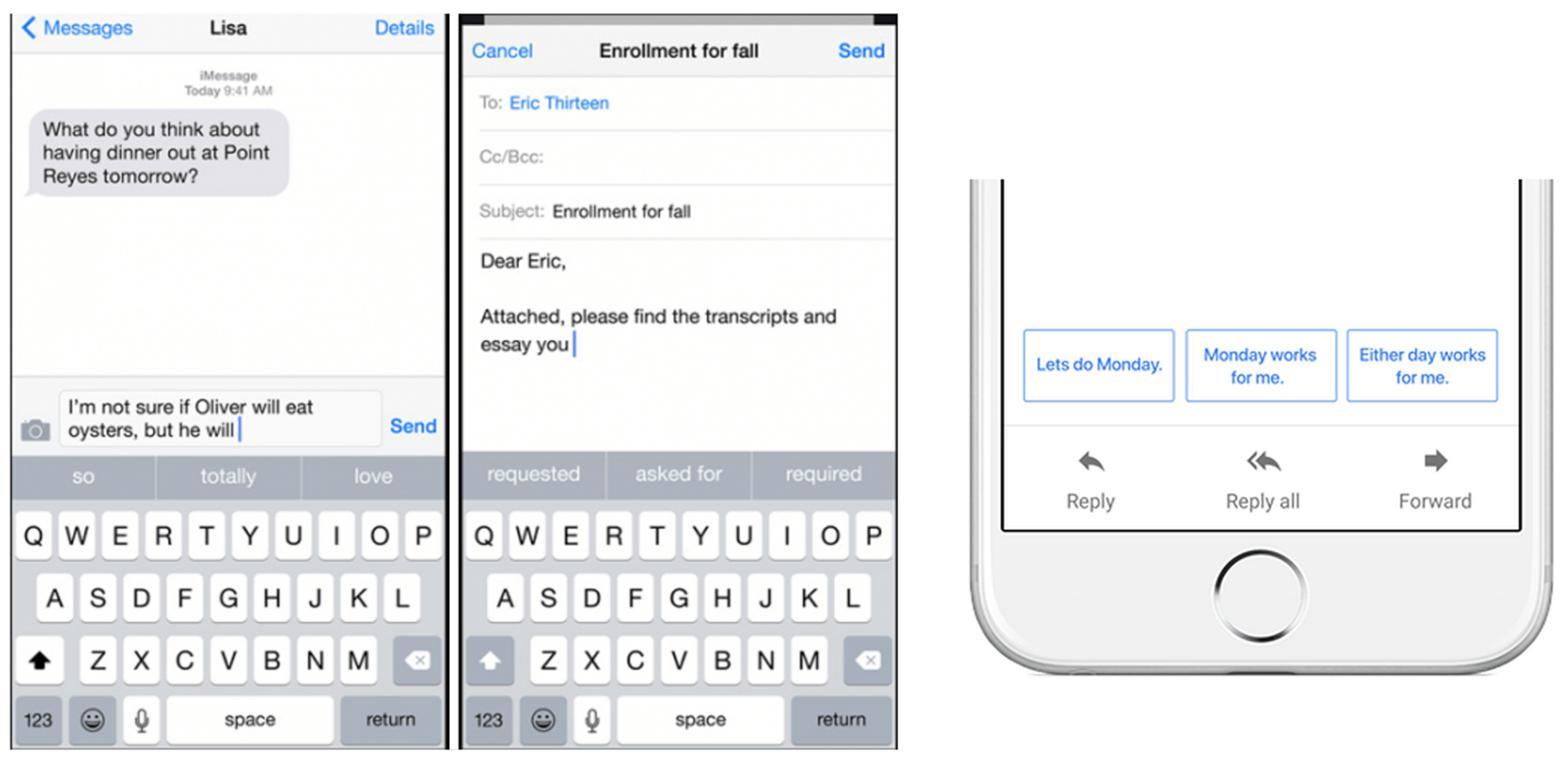
\includegraphics[scale=.2]{images/text-generation}
		\caption{On the right: Google's Smart Reply for emails}
	\end{figure}
\end{frame}

\begin{frame}{Natural Language Processing (6/8)}
	\begin{itemize}
		\item Text Classification
		
		\begin{itemize}
			\item<2-> Sentiment recognition			
			\begin{tabular}{lcl}
				\onslide<3-> "The food was good"     & $\longrightarrow$ & 
\includegraphics[scale=.25]{four-stars}	\\
				\onslide<4-> "Service was horrible"  & $\longrightarrow$ & 
\includegraphics[scale=.25]{one-star}                      
			\end{tabular}
		
		\bigskip
			\item<5-> Spam/Hoax filtering			
			
		\bigskip	
			\item<6-> News article classification into: politics, business, sports, and so on.
		\end{itemize}		
	\end{itemize}
\end{frame}


\begin{frame}{Natural Language Processing (7/8)}
	\begin{itemize}
		\item \textbf{Machine translation} 	\\
	\textbf{Contoh 1}:\\
"AI adalah listrik baru" $\Longrightarrow$ "AI is new electricity"

\bigskip
\textbf{Contoh 2}:
\begin{figure}[!ht]
	\centering
	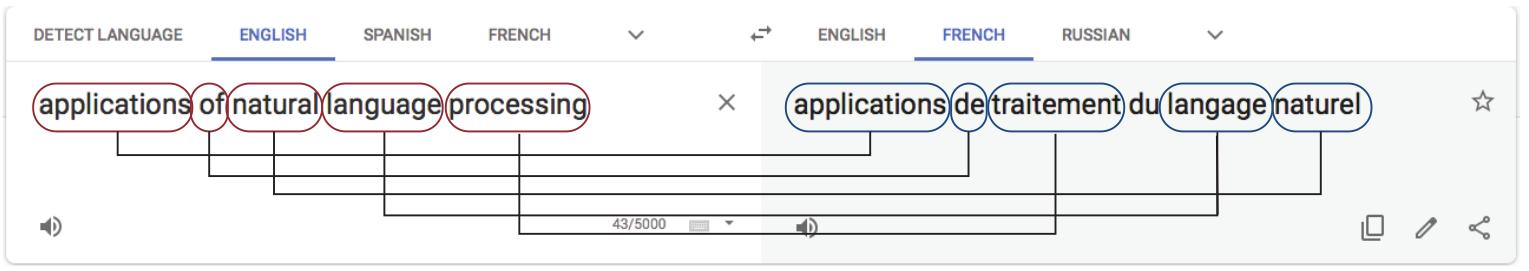
\includegraphics[scale=.2]{images/phrase-translation}
	\caption{Phrase translation between English and French}
\end{figure}
	\end{itemize}
\end{frame}

\begin{frame}{Natural Language Processing (8/8)}
	\begin{itemize}
		\item \textbf{Spell dan grammar checking}
	\end{itemize}
	\begin{figure}[!ht]
		\centering
		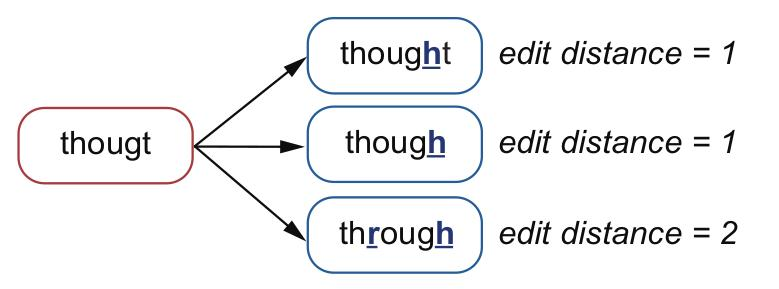
\includegraphics[scale=.2]{images/edit-distance}
		\caption{Possible corrections for the misspelling \textit{thougt}}
	\end{figure}
\end{frame}


\begin{frame}{NLP: Speech (1/2)}
	\begin{center}
		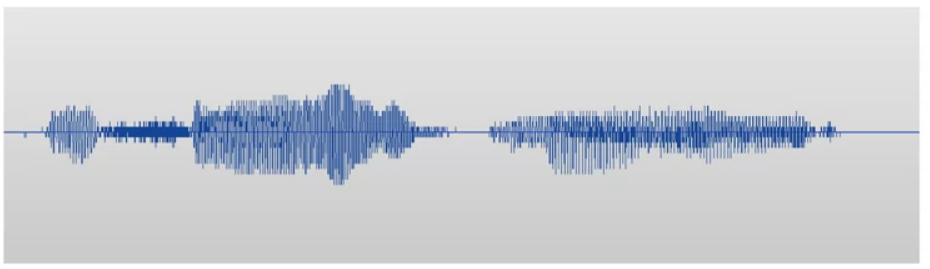
\includegraphics[scale=.25]{speech-1}
	\end{center}
	\begin{itemize}
		\item Speech recognition (speech-to-text) \\
		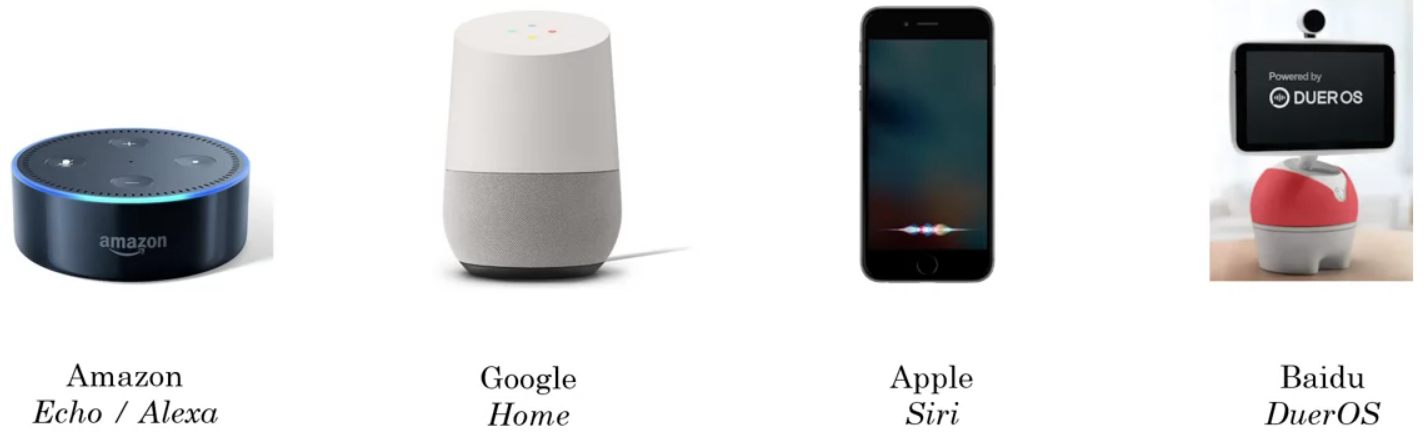
\includegraphics[scale=.2]{smart-speakers}
		\item<2-> Trigger word/wakeword detection \\
		Audio $\longrightarrow$ "Hey device"? (0/1)
	\end{itemize}
\end{frame}

\begin{frame}{NLP: Speech (2/2)}
	\begin{itemize}
		\item Speaker ID

		\bigskip

		\item<2-> Speech synthesis (text-to-speech, TTS)
		\begin{center}
			\texttt{The quick brown fox jumps over the lazy dog.}	
		\end{center}						
	\end{itemize}
\end{frame}

\begin{frame}{Times Series Forecasting (1/3)}
\begin{figure}[!ht]
		\centering
		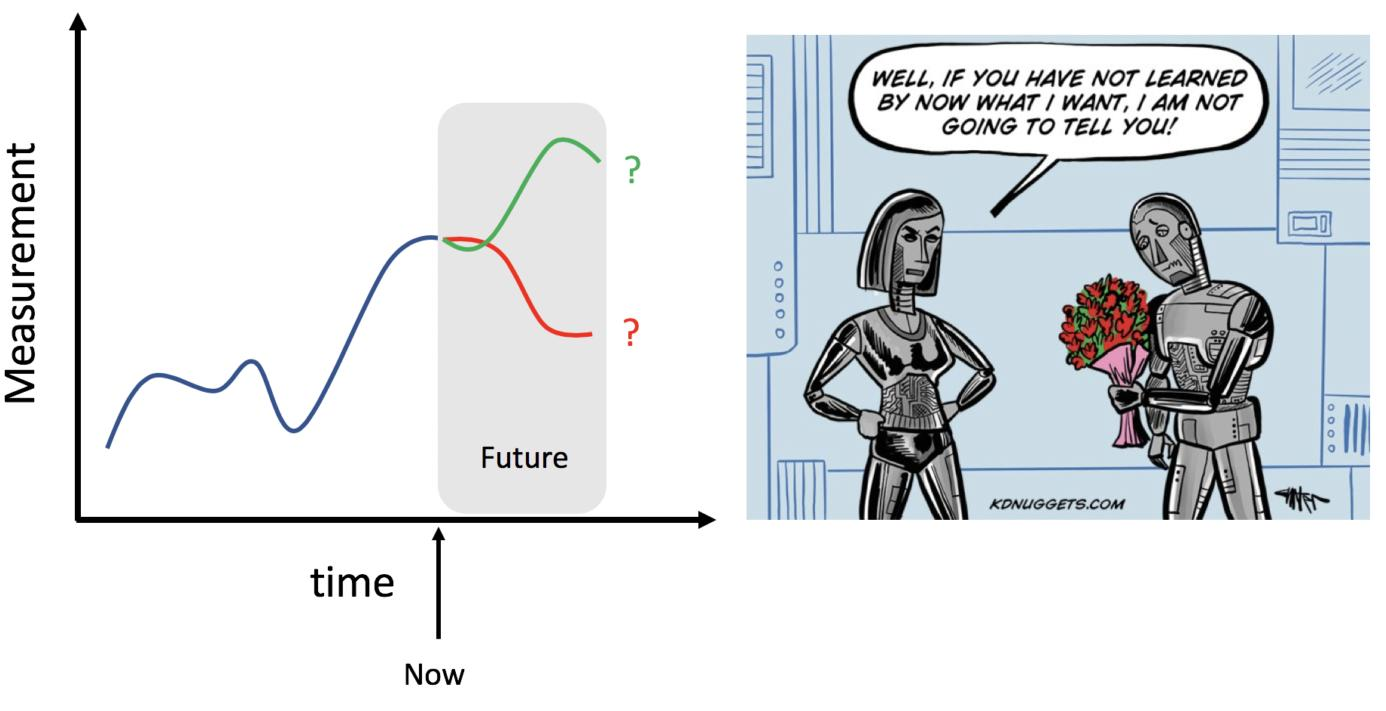
\includegraphics[scale=.25]{images/time-series-forecasting}
	\end{figure}		
\end{frame}

\begin{frame}{Times Series Forecasting (2/3)}
	\onslide<2->{Forecasting has fascinated people for thousands of years, sometimes being considered a \textit{sign of divine inspiration}, and sometimes being seen as \textit{a criminal activity} \citep{hyndman2021forecasting}.}
	\begin{figure}[!ht]
		\centering
		\includegraphics<3->[scale=.5]{fourexamples-time-series}
	\end{figure}		
\end{frame}

\begin{frame}{Times Series Forecasting (3/3)}
	This is an example of a time series which is decomposed by classical decomposition.
	\begin{figure}[!ht]
		\centering
		\includegraphics<2->[scale=.4]{classical-empl-1}
	\end{figure}		
\end{frame}

\begin{frame}{Times Series Forecasting (4/3)}
	This is an example of a time series which is decomposed by a better decomposition, X-11.
	\begin{figure}[!ht]
		\centering
		\includegraphics<2->[scale=.4]{x11-1}
	\end{figure}		
\end{frame}

\begin{frame}{Times Series Forecasting (5/3)}
	\begin{center}
	
\includegraphics[scale=.25]{images/prophet-symbol}
	\end{center}
	Salah satu algoritma untuk forecasting time series yang populer adalah \href{https://facebook.github.io/prophet/}{\textcolor{orange}{\textbf{Facebook Prophet}}} .	
	\begin{center}
		\includegraphics[scale=.35]{images/facebook-prophet-model}
	\end{center}	
\end{frame}

\begin{frame}{Reinforcement learning (1/3)}
	\begin{center}
		\includegraphics[scale=.325]{reinforcement-learning}
	\end{center}
	Use a "reward" signal to tell the AI when it is doing well or poorly. It automatically learns to maximize its rewards. \\
	(Contoh: \href{https://drive.google.com/file/d/19Zb2hjhyJ6lEUXo_OHQ0RSLrKSf6188x/view?usp=sharing}{\textcolor {orange} {\textbf{Stanford Autonomous Helicopter}} }).
\end{frame}

\begin{frame}{Reinforcement learning (2/3)}
	\begin{center}
		\includegraphics[scale=.325]{reinforcement-learning-2}
	\end{center}
	Use a "reward" signal to tell the AI when it is doing well or poorly. It automatically learns to maximize its rewards.
	(Contoh: \href{https://drive.google.com/file/d/1Bia4pGf2m1lg9Fd8Suu732Hz471nUg6j/view?usp=sharing}{\textcolor {orange} {\textbf{AlphaGo is beating Humanity}}})
\end{frame}

\begin{frame}{Reinforcement learning (3/3)}
	Dapatkah robot belajar bergerak di alam bebas? \\
	Dengan implementasi yang tepat, \textit{it can be a walk in the park} \citep{smith2022awalk}.
	
	\bigskip
	Link Video is \href{https://drive.google.com/file/d/1UE8JdqxJxpUn9McbEbfnRQXDLV9Pkmwl/view?usp=sharing}{\textcolor{orange}{\textbf{here}}}
\end{frame}

\begin{frame}{GANs (Generative Adversarial Network) (1/3)}
	\begin{center}
		Synthesize new images from scratch~\citep{karras2017progressive} (\href{https://drive.google.com/file/d/12kyeMlwG7geHo3WzO9wOo00n53LBOvpj/view?usp=sharing}{\textcolor{orange}{\textbf{GANs in Action}}})
	\end{center}
	\begin{center}
		\includegraphics[scale=.25]{GANs}
	\end{center}			
\end{frame}

\begin{frame}{GANs (Generative Adversarial Network) (2/3)}
	\textbf{GauGan} won a 2019 PopSci Magazine "Best of What's New Award" in the engineering category.
	
	\bigskip
	Developed by NVIDIA researchers in 2019, GauGAN is the first AI model that can produce complex images with only a few brushstrokes. 
	
	\bigskip
	Video Link is \href{https://twitter.com/NVIDIAAIDev/status/1201907407242153986}{\textcolor{orange}{\textbf{here}} }.
	
	\bigskip
	Aplikasi yang mirip: \href{https://affinelayer.com/pixsrv/?utm_source=pocket_reader}{\textcolor{orange}{\textbf{Image-to-Image Demo}}}	
\end{frame}

\begin{frame}{GANs (Generative Adversarial Network) (3/3)}
	\begin{itemize}
		\item Using AI to generate fashion by utilizing DALL-E. \\
		Video Link is \href{https://drive.google.com/file/d/1xrvBm1TKbGASN8CApdZkgL8sP5aXW2T_/view?usp=sharing}{\textcolor{orange}{\textbf{here}} }.
		
		\bigskip
		\item DALL-E: Introducing Outpainting \\
		Extend creativity and tell a bigger story with DALL-E images of any size. \\
		Video Link is \href{https://drive.google.com/file/d/1mJzmS_tayjQWHqwH9WyqvOdv9NGkOBMs/view?usp=share_link}{\textcolor{orange}{\textbf{here}} }.		
	\end{itemize}	
\end{frame}

\begin{frame}{AI Computing Platform}
	\begin{figure}[!ht]
		\centering
		\includegraphics[scale=.18]{images/peta-topik-huawei-ai}
	\end{figure}				
	Link Video: \href{https://drive.google.com/file/d/1e94HC381qGUsyLEfsxpE5o4btTd59HWZ/view?usp=sharing}{\textcolor{orange}{\textbf{here}}} \\
	Huawei HCIA-AI certification : \st{\$200} \textbf{\$0}.	
\end{frame}



\begin{frame}{Mata Kuliah-Mata Kuliah Jalur Peminatan \textit{AI Specialist}}
	\begin{enumerate}
		\item \textit{Computer Vision}
		\bigskip
		\item \textit{Natural Language Processing}
		\bigskip
		\item \textit{Time Series Forecasting}
		\bigskip
		\item \textit{Reinforcement Learning}
		\bigskip		
		\item \textit{AI Computing Platform}
	\end{enumerate}	
\end{frame}

%\noindent\fbox{%
%    \parbox{\textwidth}{%
%        The quick brown fox jumps right over the lazy dog. 
%    }%
%}











%\begin{frame}{Blocks}
%\begin{block}{Block Title}
%You can also highlight sections of your presentation in a block, with it's own title
%\end{block}
%\begin{theorem}
%There are separate environments for theorems, examples, definitions and proofs.
%\end{theorem}
%\begin{example}
%Here is an example of an example block.
%\end{example}
%\end{frame}


% All of the following is optional and typically not needed. 
\appendix
\section<presentation>*{\appendixname}
\subsection<presentation>*{For Further Reading}

\begin{frame}[allowframebreaks]
  \frametitle<presentation>{Daftar Pustaka}
    {\footnotesize
    \bibliographystyle{apalike}
    \bibliography{references}
    }    
\end{frame}




%\makeatletter % to change template
%    \setbeamertemplate{headline}[default] % not mandatory, but I though it was better to set it blank
%    \def\beamer@entrycode{\vspace*{-\headheight}} % here is the part we are interested in :)
%\makeatother

\begin{frame}[plain]
		\centering\includegraphics[scale=0.5]{Logo-Maranatha-Untuk-Belakang-02}	
\end{frame}

\end{document}


